% Version 3.1 December 2024 Springer Nature journal article template
% Manuscript content transferred from the author's original draft without prose edits.
\documentclass[pdflatex,sn-mathphys-num]{sn-jnl}

\usepackage{graphicx}
\graphicspath{{figures/}}
\usepackage{float}
\usepackage{amsfonts,amsmath,amssymb,amsthm}
\usepackage{xcolor}
\usepackage{url}

\theoremstyle{thmstylethree}
\newtheorem{definition}{Definition}
\theoremstyle{thmstyleone}
\newtheorem{assumption}{Assumption}
\newtheorem{proposition}{Proposition}
\newtheorem{corollary}{Corollary}

\newcommand{\ELC}{\mathrm{ELC}}
\newcommand{\TE}{\mathsf{T}}
\newcommand{\Xcur}{\mathcal{X}_{d,\tau}^{\ELC}}
\newcommand{\Xnext}{\mathcal{X}_{d,\tau+1}^{\ELC}}
\newcommand{\Xprev}{\mathcal{X}_{d,\tau-1}^{\ELC}}
\newcommand{\Xhist}{\mathcal{X}_{d,\tau}^{\ELC,(k)}}
\newcommand{\Xoldhist}{\mathcal{X}_{d,\tau-k}^{\ELC,(r)}}
\newcommand{\Xfullpast}{\mathcal{X}_{d,\tau}^{\ELC,(-\infty)}}
\newcommand{\Proc}{\mathbf{x}_{d',t_{l'}(\tau)}^{[l']}}
\newcommand{\ProcSeg}{\mathbf{x}_{d',\mathbf{s}_{l'}^{(m_{l'})}(\tau)}^{[l']}}
\newcommand{\CandProcSeg}{\mathbf{x}_{d,\mathbf{s}_{l'}^{(m_{l'})}(\tau)}^{[l']}}
\newcommand{\ProcOne}{\mathbf{x}_{d',t_{l'}(\tau)}^{[l']}}
\newcommand{\FocalProc}{\mathbf{x}_{d,\mathbf{s}_{l}^{(m_l)}(\tau)}^{[l]}}
\newcommand{\FocalBaseline}{\mathcal{X}_{d,\tau}^{\ELC\setminus\{[l]\},(k)}}
\newcommand{\FocalSupport}{\mathcal{X}_{d,\tau}^{\ELC\setminus\{[l]\}}}
\newcommand{\LowOne}{\mathbf{x}_{d,\mathbf{s}_{l_1}^{(m_{l_1})}(\tau)}^{[l_1]}}
\newcommand{\LowTwo}{\mathbf{x}_{d,\mathbf{s}_{l_2}^{(m_{l_2})}(\tau)}^{[l_2]}}
\newcommand{\Red}{\operatorname{RED}}
\newcommand{\Unq}{\operatorname{UNQ}}
\newcommand{\Syn}{\operatorname{SYN}}
\newcommand{\Suff}{\operatorname{SUFF}}
\newcommand{\FocalNext}{\mathbf{x}_{d,\mathbf{s}_{l}(\tau+1)}^{[l]}}
\newcommand{\LowerTargetNext}{\mathbf{x}_{d,\mathbf{s}_{a}(\tau+1)}^{[a]}}
\newcommand{\FocalHist}{\mathbf{x}_{d,\mathbf{s}_{l}^{(k)}(\tau)}^{[l]}}
\newcommand{\FocalOldHist}{\mathbf{x}_{d,\mathbf{s}_{l}^{(r)}(\tau-k)}^{[l]}}
\newcommand{\LineagePath}{\left\{\mathcal{X}_{d,\tau}^{\ELC}\right\}_{\tau\in\mathcal{E}}}
\newcommand{\AltLineagePath}{\left\{\widetilde{\mathcal{X}}_{d,\tau}^{\ELC}\right\}_{\tau\in\mathcal{E}}}
\newcommand{\PopPath}{\left\{\mathcal{X}_{d,\tau}^{\ELC}\right\}_{d\in\mathcal{D}_{\tau},\,\tau\in\mathcal{E}}}
\newcommand{\AltPopPath}{\left\{\widetilde{\mathcal{X}}_{d,\tau}^{\ELC}\right\}_{d\in\mathcal{D}_{\tau},\,\tau\in\mathcal{E}}}

\raggedbottom

\begin{document}

\title[An Information Theory of Extended Heredity]{An Information Theory of Extended Heredity}

\author*[1]{\fnm{Nayely} \sur{V\'elez-Cruz}}\email{nvelezcr@asu.edu}
\author[1,2,3]{\fnm{Manfred D.} \sur{Laubichler}}\nomail

\affil*[1]{\orgdiv{School of Complex Adaptive Systems}, \orgname{Arizona State University}, \orgaddress{\city{Tempe}, \state{AZ}, \country{USA}}}
\affil[2]{\orgname{Max Planck Institute of Geoanthropology}, \orgaddress{\city{Jena}, \country{Germany}}}
\affil[3]{\orgname{Santa Fe Institute}, \orgaddress{\city{Santa Fe}, \state{NM}, \country{USA}}}

\abstract{Contemporary evolutionary biology recognizes the role of multiple systems of inheritance in driving developmental and evolutionary change. As such, the repertoire of factors that are potential contributors of hereditary information has expanded beyond genes to include those ranging from epigenetic to ecological and cultural systems. However, as the range and diversity of factors implicated in heredity expand, it becomes increasingly difficult to determine which factors genuinely count as hereditary rather than merely serving as life-enabling conditions, such as temperature or oxygen, as well as how their informational contributions should be characterized and compared quantitatively. Moreover, the informational contributions of such factors are contingent on the system through which hereditary inputs are interpreted and made meaningful-- that is the next-generation organism, necessitating measures which explicitly account for this context-dependency. To address these challenges, we introduce an information-theoretic framework for evaluating hereditary information within our previously developed Extended Life Cycle (ELC), in which the organism is understood as its ELC. The ELC provides a mathematical representation of the meaning-making system through which hereditary inputs are generated, transmitted, and distributed throughout a multilevel complex biological system while linking development, heredity, reproduction, and evolutionary change within a unified formalism. We distinguish hereditary factors from life-enabling conditions based on whether they stand in a relation of mereological dependence with the next-generation ELC. We then characterize the magnitude, intergenerational stability, and distribution of these contributions throughout multiple levels of organization. Next, we identify hereditary units associated with phenotypic variants by assessing whether interventions on a factor increase the probability that the variant is reconstructed and quantifying its causal specificity via Fisher information. Finally, we identify complex units of inheritance when the preceding criteria are met by multiple factors and information about a phenotypic variant is available synergistically from those factors, as determined using partial information decompositions. We demonstrate via simulation how hereditary contributions can be evaluated without assigning explanatory priority to any particular system of inheritance a priori.}
% Original draft date retained as source metadata.
\date{August 2026}

\maketitle

\section{Introduction}
In contemporary evolutionary biology, there is an increasing recognition of the importance of multiple systems of inheritance in influencing developmental and evolutionary outcomes. These developments have renewed attention to some of the earliest and most fundamental questions about heredity: What is actually passed down across generations that is necessary for constructing an organism? What are the causes of parent-offspring resemblances? Which hereditary factors are the causes of particular phenotypic variants? At their core, these questions are about how hereditary information is constituted, transmitted, and causally expressed. Research on extended heredity has expanded the range of hereditary factors beyond genes to include epigenetic factors, ecological niches, maternal provisioning, knowledge, culture, and behavior as sources of hereditary information \cite{bonduriansky2020extended}. Within developmental systems theory (DST), this is made explicit in form of the parity thesis, according to which genetic and non-genetic factors should not be assigned different explanatory status a priori with respect to their causal roles in heredity and development. However, this expanded conception of heredity creates a foundational problem. As the range and diversity of factors implicated in heredity expands, it becomes increasingly difficult to determine which factors genuinely count as hereditary and how their contributions should be characterized and compared. Principled criteria for identifying and characterizing hereditary contributions across different systems of inheritance are therefore necessary for heredity to remain an empirically discriminating concept capable of addressing these fundamental questions within extended evolutionary theory.

Developing such criteria presents several challenges. One is in distinguishing genuine, or “true,” hereditary factors from life-enabling conditions. Although an expanded range of factors is now recognized as consequential for development and evolution, some \cite{pontarotti2015extended, shea2007representation, levy2011information} argue that the parity thesis is overly inclusive by claiming that it makes essentially no distinction between hereditary factors and general conditions such as the presence of sunlight or oxygen. A second challenge lies in determining how the contributions of those factors should be characterized and compared. Even among “true” hereditary factors, the magnitude of their contributions to phenotypic variation along with the intergenerational stability of these contributions may differ substantially in a system-dependent manner \cite{moore2019mothers,yang2020msh1,shahmohamadloo2025transgenerational}. A third challenge is that hereditary factors may interact in nonlinear and non-additive ways, such that their joint contribution cannot be inferred from their individual contributions considered in isolation \cite{jablonka2019systemic,martinez2018multimodal}. Although such non-additivity is familiar from models of epistasis, broadening the scope of heredity to include multiple inheritance systems introduces interactions among hereditary factors transmitted through different channels. A final challenge is that the influence of a hereditary factor or set of factors can vary across both developmental and evolutionary timescales. For example, the influence of a hereditary factor may vary across development and the organismal life cycle as its activity or contribution changes between life-history stages \cite{bober1991muscle,gutzwiller2015dynamics,todorov2024stage}. Across generations, the influence of a hereditary factor may likewise vary or remain latent until particular conditions arise, as illustrated by cryptic genetic variation \cite{paaby2014cryptic} and stress-induced transgenerational effects \cite{saavedra2013chronic}. Taken together, these challenges require criteria that determine which factors qualify as hereditary, quantify the magnitude and intergenerational stability of their contributions, establish whether those contributions arise independently or through irreducible interactions among factors, and quantify how their contributions change across multiple timescales.

At the same time, these challenges more fundamentally reveal that hereditary information is context-dependent, challenging code-biological views that treat hereditary information as an intrinsic property of a sequence \cite{maekivi2026methodological}. Instead, information arises through the interpretation of a hereditary factor by a system, such that it becomes meaningful for development, survival, and reproduction within a generation and, in the case of adaptive evolution, evolutionarily meaningful across generations. Here, the meaning-making system is the next-generation organism. Yet the extended evolutionary literature often leaves the organism itself, as the meaning-making system and interpretive context, insufficiently specified. Given the central role that the organism thus serves, safeguarding heredity as an empirically discriminating concept requires specifying the organismal context relative to which hereditary factors become informational. To the extent that the organism is specified in the literature, it is often treated primarily as a developmental system. Yet the factors recognized by extended heredity can act at different levels of organization and at different stages in the life cycle, of which development is a part. The relevant organismal context must therefore account for the entirety of the life cycle along with its multilevel organization. Importantly, this includes reproduction, since the organism is not only the system in which hereditary factors are interpreted throughout the life cycle, but also a participant in the reproductive processes through which the resources and relations required to reconstruct the next generation are generated, maintained, and transmitted. Reproduction encompasses the multilevel and relational processes through which the organization and resources of one life cycle contribute to the reconstruction of the next \cite{etxeberria2026expanded}. The life cycle is therefore the focal nexus linking development, reproduction, heredity, and evolutionary change across generations through which a concept of the organism can be more fully specified. We previously introduced the extended life cycle (ELC) as an operationalizable, organism-centered bridge concept that, by integrating these core dimensions, replaces the organism with an extended conception of the organism-as-its-life-cycle \cite{velezcruz2026elc}. More precisely, we defined the extended life cycle (ELC), and thus the organism-as-its-life-cycle, as the specified set of intrinsic (e.g. developmental, physiological) and extrinsic (e.g. ecological, social, abiotic) processes that maintain organismal viability and reconstruct the life cycle in the next generation via development using the resources obtained from multiple inheritance systems (genetic, epigenetic, ecological, cultural) that vary in their information bearing qualities in a system-dependent manner. We also introduced a mathematical formalization of the ELC as a multilevel, multiscale complex system \cite{velez2026extended}. This formalization allows the next-generation ELC to be treated as the meaning-making system that transforms hereditary inputs into information while providing the necessary context in which information is distributed, interpreted, and made functionally, developmentally, and evolutionarily consequential. Information theory provides the mathematical language needed to address the aforementioned challenges within the formal infrastructure of the ELC.

Building on our existing mathematical formalism, we therefore develop an information-theoretic framework for identifying, quantifying, and characterizing hereditary information within the ELC as a meaning-making system. Within this framework, reproduction consists of the relational dynamics among interacting and partially overlapping ELCs through which hereditary factors are generated. Such factors qualify as genuinely hereditary, or as “true” hereditary factors, when their interpretation by the next-generation ELC alters the probability distribution over its possible states, and when the factors contribute to the ELC's recurring organization and dynamics while their own form and persistence depend, in turn, on that organization and dynamics—a reciprocal relation we refer to as mereological dependence \cite{mediano2022greater, barad2007meeting}. We define \textit{hereditary units} as those hereditary factors whose interpretation by the next-generation ELC gives rise to hereditary information about the reconstruction of a specific phenotypic variant in a temporally contingent and context-dependent manner, such that the factors increase the probability of that variant in a \textit{causally specific} manner (in the sense of \cite{griffiths2017genetic}), while their form and persistence, as with hereditary factors more broadly, are simultaneously maintained by the ELC’s recurring organization. %\textcolor{red}{The reconstructed variant may encompass the life cycle in its entirety or correspond to a specific phenotypic feature}. 
On this account, our conception of hereditary units serves as the link between reproduction, development, and evolution within extended evolutionary theory. Reproduction generates hereditary factors through relations among ELCs; during development, the next-generation ELC interprets those factors, thereby generating information used in the reconstruction of its organization, with phenotypic variants corresponding to particular features, organized subsystems, or configurations of states within the reconstructed ELC; and evolution concerns the transgenerational recurrence and modification of the phenotypic variants thereby reconstructed. As a logical consequence of our framework, we derive the concept of \textit{complex units of inheritance}, which arises when multiple inherited factors, originating from one or more individuals and multiple systems of inheritance, form a relational structure that itself functions as a hereditary unit by jointly increasing, in a causally-specific manner, the probability that a particular phenotypic variant is reconstructed in the next-generation ELC, while its form and persistence are maintained through mereological dependence on the ELC’s recurring organization. The hereditary contribution of such a complex unit cannot be reduced to that of any single constituent factor. We develop information-theoretic measures that (1) identify and quantify the predictive contributions of hereditary factors to the next-generation ELC and determine whether they stand in a relation of mereological dependence with the ELC, thereby distinguishing hereditary factors from life-enabling conditions; (2) determine how strongly and for how many generations those hereditary contributions persist; (3) determine whether multiple hereditary factors make overlapping, source-specific, or irreducibly joint contributions to the reconstruction of the next-generation ELC, corresponding respectively to redundant, unique, and synergistic information; (4) identify where within the organization of the ELC hereditary factors contribute and characterize how those contributions vary across the dynamics of its constituent levels within each generation; (5) identify configurations of hereditary factors and determine whether they jointly function as complex units of inheritance; and (6) quantify the degree to which controlled variation in a hereditary factor produces fine-grained changes in the probability distribution over reconstructed phenotypes, thereby formalizing causal specificity using Fisher information. Together, these measures make extended heredity empirically tractable through a general complex-systems framework that can be adapted to diverse biological systems. 

\section{On Hereditary Information}
The concept of hereditary information has been developed through several partially overlapping traditions, which differ in where information is localized. Is information a context-independent property inherent to a transmitted signal itself, or is information better understood as a relationally emergent phenomenon following the encounter of a signal with an organized system? This former conception reflects code-biological perspectives which posit that hereditary information containing the instructions to construct an organism is directly encoded in molecular sequences \cite{maekivi2026methodological}. One of the earliest instantiations of the code-biological understanding of hereditary information was developed by Schrodinger, who in his 1944 work \textit{What is Life}, identified chromosomes as those units containing the instructions, or "code-script," necessary for the development and functioning of an organism \cite{schrodinger2012life}. Although early theories of heredity, such as those put forth by Darwin, Mendel, and de Vries, formulated heredity largely in terms of the transmission of hereditary units or material factors associated with traits, Schr\"{o}dinger's innovation was to recast heredity in explicitly informational and physical terms, linking hereditary information to the structure of chromosomes. Francis Crick further developed this code-biological conception by defining biological information as the precise determination of molecular sequence. Information was transferred, in this sense, when the sequence of one macromolecule determined the sequence of another, as when the sequence of a nucleic acid specifies the amino-acid sequence of a protein \cite{crick1958protein, pocheville2017crick}. This recognition helped to establish teleosemantic views of genetic information, according to which genes possess semantic, or representational \cite{shea2007representation}, content because natural selection shaped them to function as reliable information storage and transmission molecules whose sequences precisely specify biologically functional products. For this reason, genes have been historically privileged as information bearers in both developmental and evolutionary explanations \cite{maynardsmith2000information}. Importantly, this code-biological sense of hereditary information excludes non-sequence-based hereditary factors that did not evolve specifically to serve a role in the stable storage and transmission of information \cite{bergstrom2011transmission}.

In the era of extended evolutionary theory, in which the recognition of multiple systems of inheritance is broadly accepted, this view is far too restrictive. Although it is accepted that nucleotide sequences contain semantic information insofar as nucleotide triplets are mapped to amino acids through a relatively arbitrary translation system, genes are not the only biological entities that exhibit specificity. Stotz and Griffiths \cite{griffiths2017genetic} extend specificity beyond genetic inheritance systems to include contributions from epigenetic and non-genetic inheritance systems, such as methylation and chromatin states, cytoplasmic factors, maternal effects, and behaviorally, ecologically, and culturally transmitted resources. More broadly, they characterize causal, or biological, specificity as the degree to which a cause exerts fine-grained control over its effects. The more precisely variations in a cause correspond to variations in its effects, the greater its causal specificity. 

Yet, such specificity, and, more generally, the transformation of biological inputs into biological information, is context-dependent. How biological inputs become meaningful is contingent on the broader cellular, developmental, and ecological nexus in which inheritance systems operate. Such a nexus provides the necessary “meaning-making” infrastructure through which inherited inputs acquire biological significance and are incorporated into the production of particular phenotypic outcomes. Within this context, heritable inputs from multiple systems of inheritance can interact in nonlinear and non-additive ways, giving rise to what is termed “synergistic” information. Synergistic information emerges only from the joint interaction of multiple inputs within a meaning-making system and cannot be reduced to the contributions of those inputs considered individually. Moreover, from a developmental or embryological perspective, hereditary information neither pre-exists in sequences nor in broader heritable factors, but is instead actively created and distributed through dynamic ontogenetic processes, as developmental inputs are transformed into outputs that, in turn, become inputs into subsequent stages of development \cite{keller2009rethinking}. This is particularly apparent in gene regulatory networks (GRNs), which successively transform diverse inputs into phenotypic outputs, with each stage selecting from a set of possible outcomes that are not determined in advance \cite{calcott2014creation}. These processes not only occur during development, but throughout the entirety of the extended life cycle (ELC), which is the meaning-making system through which organisms undergo development, interact with other organisms, engage in decision-making processes, and participate in reproduction. 
 
The idea of meaning-making, or semiosis, refers to the process by which organisms actively and non-deterministically produce and interpret signs \cite{wolfe2026organisms}. Semiosis captures the context-dependence of information by foregrounding the organization of the interpretive system in the individual and collective decision-making processes that give meaning to signs. This non-deterministic process of interpretation lends itself to a formal probabilistic account of semantic content. More specifically, under the natural meaning of information, the information an event carries in relation to other events in the world can be identified with the change its occurrence produces in the probability distribution over the possible states of those events \cite{isaac2019semantics}. Within the ELC, such a probabilistic interpretation represents the possible phenotypic states of a complex biological system at each point in time as a probability distribution that changes over its temporal progression, analogous to the probabilistic epigenetic perspective introduced in \cite{rama2026probabilistic}. As hereditary inputs are used and reused throughout the ELC, they successively alter these probability distributions, with each change contingent on the outcomes of preceding stages. Therefore, one or more hereditary factors can be said to contain hereditary information when, within the context of the ELC, they alter the probability distribution over potential phenotypic states, thereby making particular outcomes more or less likely \cite{scarantino2015information}. In this sense, meaning-making within the ELC is formalized as the context-dependent change in state probability distributions that results from the interpretation of hereditary inputs.

However, while this probabilistic interpretation captures the context-dependence of hereditary information, it is insufficient on its own for connecting heredity to evolution. First, this view alone cannot establish the functional consequences of changes in state probability distributions, a limitation that becomes especially important if heredity is to be connected to adaptive evolution. Second, \cite{veigl2022rethinking} argues that connecting heredity to evolution requires accounting for descent with modification, whereby inheritance generates parent-offspring resemblance while permitting variation across generations. Therefore, a hereditary unit must cause, or be associated with, the reconstruction of a specific phenotypic variant by increasing the probability of that variant in a causally-specific manner. Causal specificity becomes a necessary property as merely altering the distribution of possible phenotypes does not establish that a factor contributes to the reconstruction of any particular variant; variations in the factor must correspond systematically to variations in the reconstructed phenotype. Furthermore, requiring a hereditary unit to contribute causally and specifically to the reconstruction of a phenotypic variant aligns with organizational approaches to heredity, which understand inheritance as the intergenerational reconstruction of a system’s functional organization \cite{montevil2015biological}. On this account, a factor is heritable insofar as it contributes to the reconstruction of the system’s organization and, as a constitutive functional constraint, participates in organizational closure, whereby it contributes to the maintenance of that organization while its own maintenance depends, in turn, on the organization of the system \cite{pontarotti2015extended,mossio2022conserving}. This organizational understanding of inheritance is consistent with Jablonka’s \cite{jablonka2002information} account of biological information as involving the transmission of functional organization that is reconstituted in another entity. Such reconstitution may occur either through direct material continuity or through reassembly in the absence of such continuity \cite{veigl2022rethinking}. Importantly, the requirement that hereditary factors be constitutive of the organized system helps distinguish “true” hereditary factors from merely life-enabling conditions. Within the ELC, we refer to this reciprocal part--whole relation, which is required for a hereditary factor to participate in organizational closure, as mereological dependence. By contrast, life-enabling background conditions arguably do not depend on the ELC’s organization for their own maintenance or persistence and therefore do not exhibit the same mereological dependence.
 %The organization of the system can also generate additional specificity by determining how multiple inputs are jointly interpreted, including whether their informational contributions are unique, redundant, or synergistic.

Therefore, causal specificity and organizational closure capture complementary dimensions of hereditary information. Causal specificity identifies the phenotypic variants to whose reconstruction a factor contributes, while organizational closure characterizes whether that contribution is constitutive of the organization of the ELC. Accordingly, hereditary factors contain hereditary information insofar as variations in their states alter the probability distribution over possible states of the next-generation ELC. A hereditary factor qualifies as a hereditary unit with respect to a particular phenotypic variant when it provides information about the reconstruction of that variant by increasing its probability in a causally-specific manner and is integrated into the ELC’s functional organization. Within the information-theoretic framework developed below, this mereological dependence central to organizational closure is assessed through the predictive contribution of a hereditary factor to the ELC and the predictive dependence of that factor on the ELC. The next-generation ELC serves as the meaning-making system through which these criteria will be assessed.

\section{Information Theoretic Framework}
Before introducing our information theoretic framework, it is important to first summarize the core mathematical description of the Extended Life Cycle (ELC) as described in \cite{velez2026extended}. For each entity $d$, level $l$, and level-specific time point $t_l$, let
$\mathbf{x}_{d,t_l}^{[l]} \in \mathbb{R}^{N_x^{[l]}}$ denote the latent state vector, and let
$\mathbf{y}_{d,t_l}^{[l]} \in \mathbb{R}^{N_y^{[l]}}$ denote the corresponding measurement vector. The entity $d$ may denote a biological individual, lineage, population, or another focal system, depending on the problem and data. The index $l$ corresponds to an ontological level, which may be organizational, spatial, and/or temporal in nature. For instance $l$ may refer to gene-regulatory, cell-cell communication, developmental, ecological, social, or population-level processes. For our purposes, $l$ denotes a level of organization whose dynamics take place on its own characteristic timescale. Omitting the within-level resolution index for brevity, the state transition equation is given by equation~\eqref{eq:elc-state}, and the measurement equation is given by equation~\eqref{eq:elc-measurement}:
\begin{equation}
\mathbf{x}_{d,t_l}^{[l]}
=
f_l\!\left(
\mathbf{A}_{d,t_l}^{[l]},
\mathbf{x}_{d,t_l-1}^{[l]},
\mathbf{C}_{d}^{[l]}
\left\{
\mathbf{x}_{d,s_{l'\to l}^{(m_{l'\to l})}(t_l)}^{[l']}
\right\}_{l' \neq l},
\sum_{d' \neq d}
B_{d,d',t_l}^{[l]}
\mathbf{x}_{d',t_l-1}^{[l]}
\right)
+
\mathbf{w}_{d,t_l-1}^{[l]} .
\label{eq:elc-state}
\end{equation}

\begin{equation}
\mathbf{y}_{d,t_l}^{[l]}
=
h_l\!\left(
\mathbf{x}_{d,t_l}^{[l]}
\right)
+
\mathbf{v}_{d,t_l}^{[l]} .
\label{eq:elc-measurement}
\end{equation}
Here, $f_l(\cdot)$ defines the transition dynamics at level $l$, and $h_l(\cdot)$ maps latent states to observed measurements. The matrix $\mathbf{A}_{d,t_l}^{[l]}$ represents structure internal to level $l$, such as spatial neighborhoods, gene-regulatory interactions, cell-cell communication, or other relations among components of the state vector. The mapping $\mathbf{C}_{d}^{[l]}$ represents the influence of other levels (including constraints), $\{\mathbf{x}_{d,\mathbf{s}_{l'\to l}^{(m_{l'\to l})}(t_l)}^{[l']}\}_{l' \neq l}$, on the dynamics of level $l$; for example, tissue-level organization may constrain cellular developmental dynamics, or population-level structure may constrain individual-level processes. For $l' \neq l$, $\mathbf{s}_{l'\to l}^{(m_{l'\to l})}(t_l)$ denotes the time series of length $m_{l'}$ time points in level $l'$ whose states influence the update of level $l$ at $t_l$. The interaction term $\sum_{d' \neq d} B_{d,d',t_l}^{[l]} \mathbf{x}_{d',t_l-1}^{[l]}$ represents the influence of other entities $d' \neq d$ on $d$ at the same level. Depending on the application, $B_{d,d',t_l}^{[l]}$ may encode social interactions, competition, cooperation, or another relation through which one entity affects another. For our understanding of heredity, $B_{d,d',t_l}^{[l]}$ captures reproductive interactions between individuals that contribute to the reconstruction of the ELC in the next generation. Such interactions may be level-specific or span multiple levels of biological organization. Finally, $\mathbf{w}_{d,t_l-1}^{[l]}$ represents transition noise, and $\mathbf{v}_{d,t_l}^{[l]}$ represents measurement noise. Notably, Equation~\ref{eq:elc-state} formalizes the concept of expanded reproduction introduced in \cite{etxeberria2026expanded}, in which reproduction is chiefly understood as an inherently relational process extending beyond a biological individual to include inter-individual, ecological, and developmental interactions. Let $\mathbf{s}_{l}^{(m_l)}(\tau) = (t_{l,1}, \ldots, t_{l,m_l})$ denote the ordered time series for level $l$ within generation $\tau$, where $m_l$ is the order, or length, of that time series. We may denote the ELC of of entity $d$ in generation $\tau$ as a collection of these time series, and is given by equation~\eqref{eq:elc-object}:
\begin{equation}
\mathcal{X}_{d,\tau}^{\text{ELC}}
=
\left\{
\mathbf{x}_{d,t_l}^{[l]}
\;:\;
l \in \mathcal{L},\;
t_l \in \mathbf{s}_{l}^{(m_l)}(\tau)
\right\}.
\label{eq:elc-object}
\end{equation}
Here, $\mathcal{L}$ is the set of ontological levels. The ELC object $\mathcal{X}_{d,\tau}^{\text{ELC}}$ therefore evolves through the coupled updating of its level-specific processes. %The transition functions $f_l(\cdot)$ encode within-level structure, cross-level influence, interactions among entities, and stochasticity. 
Together, Equations~\eqref{eq:elc-state} and \eqref{eq:elc-object} represent the ELC as a coupled multilevel dynamical system. 
%For mathematical and conceptual clarity, we distinguish expanded reproduction, heredity, and development based on the generations in which they occur. Reproduction occurs in generation $\tau$ and again, is a multi-agent process. Heredity is the mapping between generations $\tau$ and $\tau + 1$, and development is the process through which the next-generation organism at $\tau+1$ is reconstructed. 
For the remainder of this work, the information-theoretic framework is developed in terms of the state variables $\mathbf{x}_{d,t_l}^{[l]}$ rather than the measurement variables $\mathbf{y}_{d,t_l}^{[l]}$. The state $\mathbf{x}_{d,t_l}^{[l]}$ may be inferred from measurements or may correspond directly to measured biological variables, depending on the application. Throughout this work, we use $\mathbf{x}_{d,\mathbf{s}_{l}^{(m_l)}(\tau)}^{[l]}$ to refer to a level-$l$ time series or stochastic process of length $m_l$ in generation $\tau$. Note that $\mathbf{x}_{d,\mathbf{s}_{l}^{(m_l)}(\tau)}^{[l]}$ may represent one or more factors evaluated using the criteria developed below to determine whether they qualify as hereditary factors. The dynamics of the process are specified via the state transition equation in Equation~\ref{eq:elc-state}, which can be made explicit using, for instance, stochastic models for epigenetic memory \cite{bruno2026stochastic} or ecological inheritance models \cite{prigent2026ecological}.

\subsection{Information Theory Preliminaries}
Mutual information is one of the core concepts in information theory and measures how much knowing one variable reduces uncertainty, or entropy, about another. For two random variables $X$ and $Y$, the mutual information is given by Equation~\ref{eqn:mutualinfo}:
\begin{align}
\label{eqn:mutualinfo}
    I(X;Y)
    &= H(X) - H(X \vert Y)\\
    &= \mathbb{E}_{p(x,y)}
    \left[
        \log \frac{p(x \mid y)}{p(x)}
    \right].
\end{align}
Here, $H(X)$ denotes the entropy of $X$, and $H(X \mid Y)$ denotes the entropy of $X$ after observing $Y$. Their difference, $I(X;Y)$, is the reduction in uncertainty about $X$ provided by knowledge of $Y$, or the information that $Y$ contains about $X$. Equivalently, mutual information is the expected log-ratio between the conditional probability $p(x \mid y)$ and the marginal probability $p(x)$, where the expectation is taken over the joint distribution $p(x,y)$. It is also important to distinguish the average information between variables from the pointwise information associated with particular events. %Surprisal is inversely related to probability, and entropy is the expected surprisal over possible states. 
The pointwise mutual information between the events $X=x$ and $Y=y$ is given by Equation~\ref{eqn:pointwisemi}:
\begin{equation}
\label{eqn:pointwisemi}
    i(x;y)
    =
    \log
    \frac{p(x \mid y)}{p(x)}.
\end{equation}
Equation~\ref{eqn:pointwisemi} shows whether observing $Y=y$ raises, lowers, or leaves unchanged the probability of the specific event $X=x$. A positive value of $i(x;y)$ means that $p(x \mid y) > p(x)$, so knowledge of $Y=y$ increases the probability of $X=x$. A negative value of $i(x;y)$ means that $Y=y$ decreases the probability of $X=x$, and a value of zero means that $Y=y$ does not change the probability of $X=x$. Equation~\ref{eqn:pointwisemi} naturally lends itself to a Bayesian interpretation in which $p(x |y)$ is the posterior probability and $p(x)$ is the prior. Moreover,  Equation~\ref{eqn:pointwisemi} corresponds to the concept of natural meaning described in Section 2. In \cite{isaac2019semantics}, the collection of these log ratios is referred to as the s-vector and is given by Equation~\ref{eqn:s-vector}:
\begin{align}
\label{eqn:s-vector}
    \mathbf{S}(y)
    &=
    \left\langle
        \log\frac{p(x_1\mid y)}{p(x_1)},
        \log\frac{p(x_2\mid y)}{p(x_2)},
        \ldots,
        \log\frac{p(x_n\mid y)}{p(x_n)}
    \right\rangle \\
    &=
    \left\langle
        \log\frac{p(x_i\mid y)}{p(x_i)}
    \right\rangle_{i=1}^{n}.
\end{align}
Mutual information is the expectation of the pointwise quantity in Equation~\ref{eqn:pointwisemi} over the joint distribution of $X$ and $Y$, and is therefore a symmetric, undirected measure. As we are interested in information as it propagates throughout the ELC over time, we instead use a time-directed, asymmetric analogue to mutual information, that is, \textit{transfer entropy}. Transfer entropy is often used in complex systems modeling and measures how much knowing the current and/or past states of one time series reduces the uncertainty about the future state of another time series \cite{lizier2014jidt}. For two time series $\mathbf{X} = \{X_{1},...,X_{t},...,X_{t + \rho}\}$ and $\mathbf{Y} = \{Y_{1},...,Y_{t},...,Y_{t + \rho}\}$, the transfer entropy from the current state of $Y_{t}$ to the future state of $X_{t+1}$ given that we have observed the current state of $X_{t}$ is given by Equation~\ref{eqn:transferent}:
\begin{align}
\label{eqn:transferent}
    T_{Y \to X}
        &= I(X_{t+1}; Y_t \mid X_t) \\
        &= H(X_{t+1} \mid X_t) - H(X_{t+1} \mid Y_t, X_t) \\
        &= \mathbb{E}_{X_{t+1},Y_t,X_t}
        \left[
        \log
        \frac{
        p(X_{t+1} \mid Y_t, X_t)
        }{
        p(X_{t+1} \mid X_t)
        }
        \right].
\end{align}
A related quantity is information storage, which measures how much the current state of a time series reduces uncertainty about its own future state. For the time series $\mathbf{X}$, the information stored from $X_t$ to $X_{t+1}$ is given by Equation~\ref{eqn:infostorage}:
\begin{equation}
\label{eqn:infostorage}
    I(X_{t+1}; X_t) = H(X_{t+1}) - H(X_{t+1} \mid X_t).
\end{equation}
We now use these quantities to characterize information storage and transfer within the ELC and to relate them to the context-dependent processing, or interpretation, of heritable inputs. Let $\mathcal{X}_{d,\tau}^{\ELC,(k)}$ denote the current state of the ELC along with its history up to an order $k$. The coupled dynamics in Equation~\ref{eq:elc-state} induce the conditional probability distribution over the next-generation ELC $\mathcal{X}_{d,\tau+1}^{\text{ELC}}$ given $\mathcal{X}_{d,\tau}^{\ELC,(k)}$, as shown in equation~\eqref{eq:elc-transition-distribution}:
\begin{equation}
p\left(
\mathcal{X}_{d,\tau+1}^{\text{ELC}}
\mid
\mathcal{X}_{d,\tau}^{\text{ELC},(k)}
\right).
\label{eq:elc-transition-distribution}
\end{equation}
Within the ELC, information storage quantifies how much information the current state and history of the ELC provides about the next-generation ELC. This is given by Equation~\ref{infostorage}:
\begin{equation}
\label{infostorage}
I(\mathcal{X}_{d,\tau + 1}^{\ELC}; \mathcal{X}_{d,\tau}^{\ELC,(k)}) = H(\mathcal{X}_{d,\tau + 1}^{\text{ELC}}) - H(\mathcal{X}_{d,\tau + 1}^{\text{ELC}} | \mathcal{X}_{d,\tau}^{\text{ELC},(k)})
\end{equation}
Similarly, we can use transfer entropy as a measure of information transfer. Within the ELC, information transfer describes how much knowing the state or history of a hereditary factor, $\mathbf{x}^{[l]}_{d,\mathbf{s}^{(m_l)}_l(\tau)}$, reduces uncertainty about the future ELC, conditional on the current ELC  and its order-$k$ history. This is given by Equation~\ref{infotransfer}:
\begin{align}
\label{infotransfer}
&I(\mathcal{X}_{d,\tau + 1}^{\ELC\setminus\{[l]\}}; 
\mathbf{x}^{[l]}_{d,\mathbf{s}^{(m_l)}_l(\tau)} 
\mid \mathcal{X}_{d,\tau}^{\ELC\setminus\{[l]\},(k)}) \\
\nonumber
&= H(\mathcal{X}_{d,\tau + 1}^{\ELC\setminus\{[l]\}} 
\mid \mathcal{X}_{d,\tau}^{\ELC\setminus\{[l]\},(k)})
- H(\mathcal{X}_{d,\tau + 1}^{\ELC\setminus\{[l]\}} 
\mid \mathbf{x}^{[l]}_{d,\mathbf{s}^{(m_l)}_l(\tau)}, 
\mathcal{X}_{d,\tau}^{\ELC\setminus\{[l]\},(k)}).
\end{align}
Lastly, in our work, information processing refers to how the coupled dynamics of the ELC map its current state and history, together with one or more inputs, to a conditional probability distribution over possible future states. Equation~\ref{eq:elc-state} specifies the dynamics that define this mapping. An input becomes informational when conditioning on that input changes the distribution over possible future ELC states relative to the distribution conditioned on the current ELC state and its history alone, with the expected magnitude of this change quantified by Equation~\ref{infotransfer}. Within the broader criteria developed below, meaning relative to the next-generation ELC is established by whether conditioning on an input changes the probabilities assigned to possible future states and, if so, which states become more or less probable given the current ELC state and history. Although the specific biological mechanisms underlying these meaning-making processes differ across levels of biological organization, the ELC framework accommodates this diversity through its level-specific yet coupled transition dynamics while retaining a general information-theoretic formalism that applies across levels.

\subsection{Quantifying the predictive contributions of systems of inheritance} 
In this section we present general criteria to quantify the predictive contributions to the next-generation ELC of any system of inheritance whose dynamics can be modeled via the structure in Equation~\ref{eq:elc-state}. The two criteria introduced in this section operationalize mereological dependence between the inheritance process and the ELC. Criterion 1 specifies when a  hereditary process contributes predictive information to the next-generation ELC, while Criterion 2 specifies when the inheritance process depends on the ELC for its maintenance and persistence, operationalized through the predictive information that the ELC provides about the future state of the process. Within this framework, an inheritance process participates in organizational closure when it is represented as a constitutive part of the ELC's state-space dynamics and satisfies both criteria for mereological dependence. These criteria help us to address two critiques of the parity thesis, the first being that not all hereditary inputs will be of equal importance for the reconstruction of the next-generation ELC, and the second relating to the indistinguishability between life-enabling background conditions and genuine hereditary factors in the sense of \cite{veigl2022rethinking}. %Accordingly, we develop several criteria by which to assess the informational contributions of various systems of inheritance, as well as to help determine whether a hereditary contribution is a genuine genuine hereditary unit.  %Biological heredity can be broadly conceived of as the intergenerational transfer of resources that are used to reconstruct an organism, or for our purposes, the ELC in the next generation. In this sense, hereditary information is tied not only to the transmission of factors that are necessary for the intergenerational continuity of organization, but also to the reconstruction of specific phenotypic variants within the ELC. Information can be transmitted from a range of inheritance channels, and 

 

%Before introducing the criterion, we first need to make a clarification regarding the notation used in this section. There are instances in which the  inheritance process will be a priori defined as part of the ELC's organization. In such cases, one will need to exclude the  inheritance process from the ELC definition, which we do using the following notation $\mathcal{X}_{d,\tau}^{\ELC\setminus\{[l]\}}$. If the  inheritance process is not a priori defined as part of the ELC, then we may omit the exclusion notation and simply use $\mathcal{X}_{d,\tau}^{\ELC}$. For the remainder of the section, we will assume the former case and therefore use $\mathcal{X}_{d,\tau}^{\ELC\setminus\{[l]\}}$. 

\paragraph{Criterion 1: Hereditary factors contribute predictive information to the next-generation ELC.}
One or more hereditary factors contribute hereditary information when they alter the state probability distribution of the next-generation ELC beyond what is predicted by the current ELC and its order-$k$ history. Specifically, the  inheritance process contributes hereditary information when
$p\!\left(
\mathcal{X}_{d,\tau+1}^{\ELC\setminus\{[l]\}}
\mid
\mathbf{x}^{[l]}_{d,\mathbf{s}^{(m_l)}_l(\tau)},
\mathcal{X}_{d,\tau}^{\ELC\setminus\{[l]\},(k)}
\right)
\neq
p\!\left(
\mathcal{X}_{d,\tau+1}^{\ELC\setminus\{[l]\}}
\mid
\mathcal{X}_{d,\tau}^{\ELC\setminus\{[l]\},(k)}
\right)
$
for at least one combination of
$\mathbf{x}^{[l]}_{d,\mathbf{s}^{(m_l)}_l(\tau)}$
and
$\mathcal{X}_{d,\tau}^{\ELC\setminus\{[l]\},(k)}$
that occurs with positive probability. The expected magnitude of this distributional change is quantified by the transfer entropy in Equation~\eqref{eq:heredity-total--in-elc}:
\begin{align}
&I\!\left(
\mathcal{X}_{d,\tau+1}^{\ELC\setminus\{[l]\}};
\mathbf{x}^{[l]}_{d,\mathbf{s}^{(m_l)}_l(\tau)}
\mid
\mathcal{X}_{d,\tau}^{\ELC\setminus\{[l]\},(k)}
\right)
\notag\\
&=
H\!\left(
\mathcal{X}_{d,\tau+1}^{\ELC\setminus\{[l]\}}
\mid
\mathcal{X}_{d,\tau}^{\ELC\setminus\{[l]\},(k)}
\right)
-
H\!\left(
\mathcal{X}_{d,\tau+1}^{\ELC\setminus\{[l]\}}
\mid
\mathbf{x}^{[l]}_{d,\mathbf{s}^{(m_l)}_l(\tau)},
\mathcal{X}_{d,\tau}^{\ELC\setminus\{[l]\},(k)}
\right)
\notag\\
&=
\mathbb{E}\!\left[
D_{\mathrm{KL}}\!\left(
p\!\left(
\mathcal{X}_{d,\tau+1}^{\ELC\setminus\{[l]\}}
\mid
\mathbf{x}^{[l]}_{d,\mathbf{s}^{(m_l)}_l(\tau)},
\mathcal{X}_{d,\tau}^{\ELC\setminus\{[l]\},(k)}
\right)
\middle\|
p\!\left(
\mathcal{X}_{d,\tau+1}^{\ELC\setminus\{[l]\}}
\mid
\mathcal{X}_{d,\tau}^{\ELC\setminus\{[l]\},(k)}
\right)
\right)
\right]
>0.
\label{eq:heredity-total--in-elc}
\end{align}
In practical applications, it may be useful to define or infer a threshold $\epsilon>0$ such that the estimated information must exceed $\epsilon$ to be counted as a predictive contribution to the next-generation ELC. It may also be the case that an  inheritance process contributes not only in the immediate next generation, but also at a later generational horizon. To account for this, the same criterion can be evaluated at some future generation $\rho >1$ via Equation~\ref{eq:heredity-total--horizon}:
\begin{equation}
\label{eq:heredity-total--horizon}
I\!\left(
\mathcal{X}_{d,\tau+\rho}^{\ELC\setminus\{[l]\}};
\mathbf{x}^{[l]}_{d,\mathbf{s}^{(m_l)}_l(\tau)}
\mid
\mathcal{X}_{d,\tau}^{\ELC\setminus\{[l]\},(k)}
\right)>0.
\end{equation}

\paragraph{Criterion 2: Dependence of the  inheritance process on the ELC.}
The inheritance process depends on the ELC when its maintenance and persistence depends on the organization of the ELC. Together with the predictive contribution established in Criterion 1, this helps distinguish genuine hereditary factors from life-enabling background conditions that may reduce uncertainty about the future ELC since the persistence of a life-enabling condition does not itself depend on the organization of the ELC. This dependence is evaluated by assessing whether the current state of the ELC, along with its order-$k$ history, transfers predictive information to the future state of the inheritance process. This condition is given by Equation~\eqref{eq:elc-to--condition}:
\begin{equation}
\label{eq:elc-to--condition}
I\!\left(
\mathbf{x}^{[l]}_{d,\mathbf{s}^{(m_l)}_l(\tau+\rho)};
\mathcal{X}_{d,\tau}^{\ELC\setminus\{[l]\},(k)}
\mid
\mathbf{x}^{[l]}_{d,\mathbf{s}^{(m_l)}_l(\tau)}
\right)>0.
\end{equation}
Importantly, Criteria 1 and 2 together operationalize mereological dependence. %Mereological dependence means that the functioning, maintenance, and temporal persistence of the whole system depend on the organization and contributions of its components, while the functioning, persistence, and identity of those components are possible only through their relations within the whole \cite{barad2007meeting}.

As well, the same criteria can be used to evaluate the informational contributions of one or more ELCs ($d' \neq d$), such as parents, ancestral lineages, caregivers, social partners, colony members, or other individuals whose interactions may provide predictive information about the reconstruction of the next-generation ELC of $d$. This can be computed for the ELC as a whole for any $Q$ number of ELCs $d'_1,\ldots,d'_Q$, as shown in Equation~\eqref{eq:multiple-parent-whole-elc-contribution}:
\begin{equation}
\label{eq:multiple-parent-whole-elc-contribution}
I\!\left(
\mathcal{X}^{\ELC}_{d,\tau+1};
\mathcal{X}^{\ELC}_{d'_1,\tau},
\ldots,
\mathcal{X}^{\ELC}_{d'_Q,\tau}
\mid
\mathcal{X}^{\ELC,(k)}_{d,\tau}
\right)>0,
\end{equation}
or at the subsystem-level as shown in Equation~\eqref{eq:multiple-parent-subsystem-contribution}:
\begin{equation}
\label{eq:multiple-parent-subsystem-contribution}
I\!\left(
\mathcal{X}^{\ELC}_{d,\tau+1};
\mathbf{x}^{[l]}_{d'_1,\mathbf{s}^{(m_l)}_l(\tau)},
\ldots,
\mathbf{x}^{[l]}_{d'_Q,\mathbf{s}^{(m_l)}_l(\tau)}
\mid
\mathcal{X}^{\ELC,(k)}_{d,\tau}
\right)>0.
\end{equation}

\subsubsection{Hereditary units increase the probability of specific phenotypic variants and exhibit causal specificity.}
A hereditary factor qualifies as a hereditary unit with respect to a phenotypic variant only when its contribution can be linked to the reconstruction of that specific variant in the next-generation ELC. In a given ELC, the factor must provide positive predictive information about the variant, interventions on the factor must increase the probability that the variant is reconstructed in the next-generation ELC, and interventions on the factor must exert fine-grained control over the distribution of reconstructed phenotypes (causal specificity). Let $\mathcal{V}_{d,\tau+1}$ denote a phenotypic random variable defined from the state or trajectory of the next-generation ELC, $\mathcal{X}_{d,\tau+1}^{\ELC}$, for instance, through a mapping such as  $\mathcal{V}_{d,\tau+1} = g(\mathcal{X}_{d,\tau+1}^{\ELC})$. Depending on the application, $\mathcal{V}_{d,\tau+1}$ may consist of a subset of the ELC state variables or may be computed from their values across the life cycle to represent a phenotype of interest. Let $\nu$ denote a particular realization of $\mathcal{V}_{d,\tau+1}$, corresponding to the phenotypic variant under consideration. For a continuous phenotype, a phenotypic variant may be defined as a measurable region $A_{\nu}$ of the phenotype space, such that $\mathcal{V}_{d,\tau+1} \in A_{\nu}$ defines the variant of interest. Accordingly, occurrences of $\mathcal{V}_{d,\tau+1}=\nu$ below are understood as $\mathcal{V}_{d,\tau+1}\in A_{\nu}$. 

\paragraph{Criterion 1. Positive predictive information is associated with the reconstruction of the variant.}
The hereditary factor provides positive predictive information about the reconstruction of variant $\nu$ when, given the current state and history of the ELC, the pointwise conditional log-ratio in Equation~\eqref{eq:variant-pointwise-information} is positive:
\begin{equation}
\label{eq:variant-pointwise-information}
\log
\frac{
p\!\left(
\mathcal{V}_{d,\tau+1}=\nu
\mid
\mathbf{x}^{[l]}_{d,\mathbf{s}^{(m_l)}_l(\tau)},
\mathcal{X}_{d,\tau}^{\ELC\setminus\{[l]\},(k)}
\right)
}{
p\!\left(
\mathcal{V}_{d,\tau+1}=\nu
\mid
\mathcal{X}_{d,\tau}^{\ELC\setminus\{[l]\},(k)}
\right)
}
>0.
\end{equation}
Equation~\eqref{eq:variant-pointwise-information} is positive when conditioning on the hereditary factor increases the probability that variant $\nu$ is reconstructed in the next-generation ELC. The vector of conditional log-ratios formed by evaluating Equation~\eqref{eq:variant-pointwise-information} across the possible realizations of $\mathcal{V}_{d,\tau+1}$ characterizes the semantic content, or natural meaning, of the hereditary factor relative to the next-generation ELC \cite{isaac2019semantics}.

\paragraph{Criterion 2. Hereditary units exhibit causal specificity with respect to phenotypic variants.}
Following \cite{griffiths2015measuring, griffiths2017genetic}, causal, or biological, specificity refers to the degree of fine-grained control over an effect afforded by interventions on a causal variable. To qualify as a hereditary unit, a hereditary factor must increase the probability of a variant in a causally-specific manner. Let $\boldsymbol{\theta}_x$ denote the vector of parameters governing the intervention, and let $\theta_{x,r}$ denote its $r$th component. The components of $\boldsymbol{\theta}_x$ parameterize the allowed interventions. We assume that the intervention family is differentiably parameterized by $\boldsymbol{\theta}_x$ and that the parameter value under evaluation lies in the interior of the admissible intervention space, such that sufficiently small changes in either direction are permitted. Let $\widetilde{\mathbf{x}}^{[l]}_{d,\mathbf{s}^{(m_l)}_l(\tau)}(\boldsymbol{\theta}_x)$ denote the state of the hereditary factor under an intervention parameterized by $\boldsymbol{\theta}_x$. The distribution of $\mathcal{V}_{d,\tau+1}$ under the intervention is given by Equation~\eqref{eq:variant-intervention-distribution}:
\begin{equation}
\label{eq:variant-intervention-distribution}
\begin{aligned}
&p_{\boldsymbol{\theta}_x}\left(
\mathcal{V}_{d,\tau+1}
\mid
\mathcal{X}_{d,\tau}^{\ELC\setminus\{[l]\},(k)}
\right)
\\
&\qquad =
p\left(
\mathcal{V}_{d,\tau+1}
\mid
\operatorname{do}\left(
\mathbf{x}^{[l]}_{d,\mathbf{s}^{(m_l)}_l(\tau)}
=
\widetilde{\mathbf{x}}^{[l]}_{d,\mathbf{s}^{(m_l)}_l(\tau)}(\boldsymbol{\theta}_x)
\right),
\mathcal{X}_{d,\tau}^{\ELC\setminus\{[l]\},(k)}
\right).
\end{aligned}
\end{equation}
For a component $\theta_{x,r}$ of the intervention parameter vector, the hereditary factor causally (in the Woodward interventionist sense) increases the probability that the specific variant $\nu$ is reconstructed when the factor can be changed locally in a direction that increases the probability of $\nu$. This condition is satisfied when:
\begin{equation}
\label{eq:variant-probability-increase}
\frac{\partial}{\partial \theta_{x,r}}
p_{\boldsymbol{\theta}_x}\left(
\mathcal{V}_{d,\tau+1}=\nu
\mid
\mathcal{X}_{d,\tau}^{\ELC\setminus\{[l]\},(k)}
\right)
\neq 0.
\end{equation}
The biological, or causal, specificity of the hereditary factor with respect to the reconstructed phenotype is quantified by the Fisher information matrix of the distribution in Equation~\eqref{eq:variant-intervention-distribution}, as given by Equation~\eqref{eq:variant-causal-specificity}:
\begin{equation}
\label{eq:variant-causal-specificity}
\begin{aligned}
\mathbf{F}_{x}(\boldsymbol{\theta}_x)
&=
\mathbb{E}_{
\mathcal{V}_{d,\tau+1}
\sim
p_{\boldsymbol{\theta}_x}\left(
\cdot
\mid
\mathcal{X}_{d,\tau}^{\ELC\setminus\{[l]\},(k)}
\right)
}
\Bigg[
\nabla_{\boldsymbol{\theta}_x}
\log
p_{\boldsymbol{\theta}_x}\left(
\mathcal{V}_{d,\tau+1}
\mid
\mathcal{X}_{d,\tau}^{\ELC\setminus\{[l]\},(k)}
\right)
\\
&\qquad\qquad\quad
\times
\nabla_{\boldsymbol{\theta}_x}
\log
p_{\boldsymbol{\theta}_x}\left(
\mathcal{V}_{d,\tau+1}
\mid
\mathcal{X}_{d,\tau}^{\ELC\setminus\{[l]\},(k)}
\right)^{\top}
\Bigg].
\end{aligned}
\end{equation}
The gradients in Equation~\eqref{eq:variant-causal-specificity} are taken with respect to the intervention parameters governing the hereditary factor, while $\mathcal{X}_{d,\tau}^{\ELC\setminus\{[l]\},(k)}$ is held fixed. For the component $\theta_{x,r}$ evaluated in Equation~\eqref{eq:variant-probability-increase}, the hereditary factor exhibits nonzero local causal specificity when
$
\left[
\mathbf{F}_{x}(\boldsymbol{\theta}_x)
\right]_{rr}
>0$.
The value of $\left[\mathbf{F}_{x}(\boldsymbol{\theta}_x)\right]_{rr}$ quantifies the local causal specificity associated with changes in $\theta_{x,r}$, where $[\cdot]_{rr}$ denotes the $r$th diagonal entry of the Fisher information matrix. Holding the intervention parameterization fixed, larger values indicate that small changes in $\theta_{x,r}$ produce larger changes in the distribution over the possible states of $\mathcal{V}_{d,\tau+1}$.

%\paragraph{Remark 1: Hereditary units contribute to adaptive evolution when they contribute to the success of a variant.}
%Next, we can evaluate whether a hereditary unit contributes to adaptive evolution. Let $\mathcal{V}_{d,\tau+1}$ denote the phenotype under consideration, let $\nu$ denote a particular phenotypic variant, and let $\mathcal{X}_{d,\tau+1}^{\ELC\setminus\mathcal{V}}$ denote the remaining states of the next-generation ELC outside the phenotype. The expected fitness of $\nu$, conditional on the current ELC and its order-$k$ history, is given by Equation~\eqref{eq:variant-expected-fitness}:
%\begin{equation}
%\label{eq:variant-expected-fitness}
%\overline{F}\!\left(
%\nu
%\mid
%\mathcal{X}_{d,\tau}^{\ELC,(k)}
%\right)
%=
%\sum_{\mathcal{X}_{d,\tau+1}^{\ELC\setminus\mathcal{V}}}
%p\!\left(
%\mathcal{X}_{d,\tau+1}^{\ELC\setminus\mathcal{V}}
%\mid
%\mathcal{V}_{d,\tau+1}=\nu,
%\mathcal{X}_{d,\tau}^{\ELC,(k)}
%\right)
%F\!\left(
%\nu
%\mid
%\mathcal{X}_{d,\tau+1}^{\ELC\setminus\mathcal{V}}
%\right).
%\end{equation}
%Equation~\eqref{eq:variant-expected-fitness} gives the expected fitness of the variant across the possible states of the rest of the next-generation ELC in which the variant is reconstructed. A hereditary unit contributes to adaptive evolution when it increases the probability that $\mathcal{V}_{d,\tau+1}=\nu$ is reconstructed and $\nu$ has greater expected fitness than the relevant alternative.

\subsection{Quantifying Intergenerational Stability}
Inheritance systems differ in the stability of their predictive contributions in a system-dependent manner \cite{heard2014transgenerational, quadrana2016plant}. We therefore quantify intergenerational stability as the persistence of the predictive contribution of an inheritance process across future generations. The intergenerational stability profile $\mathbf{R}^{[l]}_{d,\tau}(\rho)$ over $\rho$ future generations is given by Equation \eqref{eq:intergenerational-stability-profile}:
\begin{align}
\label{eq:intergenerational-stability-profile}
\mathbf{R}^{[l]}_{d,\tau}(\rho)
=
\left(
\begin{array}{l}
I\!\left(
X^{\ELC\setminus\{[l]\}}_{d,\tau+1};
\mathbf{x}^{[l]}_{d,\mathbf{s}_{l}^{(m_l)}(\tau)}
\mid
X^{\ELC\setminus\{[l]\},(k)}_{d,\tau}
\right),
\\[0.8em]
I\!\left(
X^{\ELC\setminus\{[l]\}}_{d,\tau+2};
\mathbf{x}^{[l]}_{d,\mathbf{s}_{l}^{(m_l)}(\tau)}
\mid
X^{\ELC\setminus\{[l]\},(k)}_{d,\tau}
\right),
\\[0.8em]
\ldots,
\\[0.8em]
I\!\left(
X^{\ELC\setminus\{[l]\}}_{d,\tau+\rho};
\mathbf{x}^{[l]}_{d,\mathbf{s}_{l}^{(m_l)}(\tau)}
\mid
X^{\ELC\setminus\{[l]\},(k)}_{d,\tau}
\right)
\end{array}
\right)
\end{align}
Equation \eqref{eq:intergenerational-stability-profile} can similarly be applied to quantify the stability of hereditary contributions from multiple systems of inheritance in addition to multiple ELCs $d' \neq d$.

\subsection{How Hereditary Information is Distributed Throughout the ELC}
Another advantage of our information-theoretic framework is its ability to quantify how hereditary information is distributed across the different levels or subsystems that comprise the ELC. Given a focal level $l$ and a hereditary factor $\mathbf{x}^{[l']}_{d,\mathbf{s}^{(m_{l'})}_{l'}(\tau)}$ at level $l'$, where $l\neq l'$, Equation~\ref{eqn:distofhereditaryinfo} quantifies the predictive information that the hereditary factor provides about the next-generation state of the focal level $l$, conditional on the current state and order-$k$ history of the ELC:
\begin{equation}
\label{eqn:distofhereditaryinfo}
T^{[l' \to l]}_{d,\tau}
=
I\left(
\mathbf{x}^{[l]}_{d,\mathbf{s}^{(m_l)}_l(\tau+1)};
\mathbf{x}^{[l']}_{d,\mathbf{s}^{(m_{l'})}_{l'}(\tau)}
\;\middle|\;
\mathcal{X}^{\mathrm{ELC}\setminus\{[l']\},(k)}_{d,\tau}
\right).
\end{equation}
Equation~\ref{eqn:distofhereditaryinfo} can then be evaluated for each focal level $l\neq l'$ in the next-generation ELC. Here, $\mathbf{s}^{(m_l)}_l(\tau+1)$ may denote, for instance, a developmental window or life-cycle phase. This allows the predictive contribution of a hereditary factor to vary across different timescales and levels of organization rather than being treated as constant.% Evaluating Equation~\ref{eqn:distofhereditaryinfo} across the focal levels identifies where the hereditary factor contributes predictive information within the ELC, rather than only asking whether it contributes to the next-generation ELC as a whole. 
The resulting level-wise distribution of predictive contributions is summarized by Equation~\ref{eqn:distofhereditaryinfo-profile}:
\begin{equation}
\label{eqn:distofhereditaryinfo-profile}
\mathbf{T}^{[l']}_{d,\tau}
=
\left(
T^{[l' \to 1]}_{d,\tau},
T^{[l' \to 2]}_{d,\tau},
\ldots,
T^{[l' \to L]}_{d,\tau}
\right).
\end{equation}

\subsection{Partial Information Decompositions of Multiple Inheritance Systems}
Of particular interest is evaluating whether different inheritance systems contribute hereditary information independently, exhibit overlap in the information they provide, or contribute information that arises only when considering the systems jointly. Partial information decomposition (PID) separates these contributions into unique, redundant, and synergistic information, respectively \cite{williams2010nonnegative, kolchinsky2022novel, lyu2026multivariate}. Redundant information refers to hereditary information about the next-generation ELC that is provided by more than one inheritance system. Unique information refers to hereditary information that is provided by one inheritance system but not by the others. Synergistic information refers to hereditary information that only becomes available when multiple inheritance systems are considered together \cite{rama2026developmental}. For any hereditary factors $\mathbf{x}^{[l_1]}_{d,\mathbf{s}^{(m_{l_1})}_{l_1}(\tau)}$ and $\mathbf{x}^{[l_2]}_{d,\mathbf{s}^{(m_{l_2})}_{l_2}(\tau)}$ originating from two inheritance systems, we can decompose the predictive information into these components as shown in Equation~\ref{PIDmultipleinheritance}:
\begin{align}
\label{PIDmultipleinheritance}
&
I\left(
\mathcal{X}^{\mathrm{ELC}\setminus\{[l_1],[l_2]\}}_{d,\tau+1};
\mathbf{x}^{[l_1]}_{d,\mathbf{s}^{(m_{l_1})}_{l_1}(\tau)},
\mathbf{x}^{[l_2]}_{d,\mathbf{s}^{(m_{l_2})}_{l_2}(\tau)}
\mid
\mathcal{X}^{\mathrm{ELC}\setminus\{[l_1],[l_2]\},(k)}_{d,\tau}
\right)
\nonumber\\
&=
\operatorname{Red}^{\mathrm{ELC}}_{\Pi}
\left(
\mathcal{X}^{\mathrm{ELC}\setminus\{[l_1],[l_2]\}}_{d,\tau+1};
\mathbf{x}^{[l_1]}_{d,\mathbf{s}^{(m_{l_1})}_{l_1}(\tau)},
\mathbf{x}^{[l_2]}_{d,\mathbf{s}^{(m_{l_2})}_{l_2}(\tau)}
\mid
\mathcal{X}^{\mathrm{ELC}\setminus\{[l_1],[l_2]\},(k)}_{d,\tau}
\right)
\nonumber\\
&\quad+
\operatorname{UI}^{\mathrm{ELC}}_{\Pi,l_1}
\left(
\mathcal{X}^{\mathrm{ELC}\setminus\{[l_1],[l_2]\}}_{d,\tau+1};
\mathbf{x}^{[l_1]}_{d,\mathbf{s}^{(m_{l_1})}_{l_1}(\tau)}
\setminus
\mathbf{x}^{[l_2]}_{d,\mathbf{s}^{(m_{l_2})}_{l_2}(\tau)}
\mid
\mathcal{X}^{\mathrm{ELC}\setminus\{[l_1],[l_2]\},(k)}_{d,\tau}
\right)
\nonumber\\
&\quad+
\operatorname{UI}^{\mathrm{ELC}}_{\Pi,l_2}
\left(
\mathcal{X}^{\mathrm{ELC}\setminus\{[l_1],[l_2]\}}_{d,\tau+1};
\mathbf{x}^{[l_2]}_{d,\mathbf{s}^{(m_{l_2})}_{l_2}(\tau)}
\setminus
\mathbf{x}^{[l_1]}_{d,\mathbf{s}^{(m_{l_1})}_{l_1}(\tau)}
\mid
\mathcal{X}^{\mathrm{ELC}\setminus\{[l_1],[l_2]\},(k)}_{d,\tau}
\right)
\nonumber\\
&\quad+
\operatorname{SI}^{\mathrm{ELC}}_{\Pi}
\left(
\mathcal{X}^{\mathrm{ELC}\setminus\{[l_1],[l_2]\}}_{d,\tau+1};
\mathbf{x}^{[l_1]}_{d,\mathbf{s}^{(m_{l_1})}_{l_1}(\tau)},
\mathbf{x}^{[l_2]}_{d,\mathbf{s}^{(m_{l_2})}_{l_2}(\tau)}
\mid
\mathcal{X}^{\mathrm{ELC}\setminus\{[l_1],[l_2]\},(k)}_{d,\tau}
\right).
\end{align}
Here, $\Pi$ denotes the PID convention used to decompose the predictive information. Equation~\ref{PIDmultipleinheritance} decomposes the total predictive information that the hereditary factors at levels $l_1$ and $l_2$ provide about the next-generation ELC, excluding those same levels from the future ELC. This partitions hereditary information into components that are redundant across both factors, unique to each factor, or synergistic and only available when the two factors are considered jointly.

For multiple hereditary factors to qualify as a complex unit of inheritance with respect to a particular phenotypic variant $\nu$, they must contribute synergistic information to the reconstruction of $\nu$. This can be evaluated by applying the PID to the focal variant as shown in Equation~\ref{PIDcomplexvariant}:
\begin{align}
\label{PIDcomplexvariant}
&
I\left(
\mathbf{1}\{V_{d,\tau+1}=\nu\};
\mathbf{x}^{[l_1]}_{d,\mathbf{s}^{(m_{l_1})}_{l_1}(\tau)},
\mathbf{x}^{[l_2]}_{d,\mathbf{s}^{(m_{l_2})}_{l_2}(\tau)}
\mid
\mathcal{X}^{\mathrm{ELC}\setminus\{[l_1],[l_2]\},(k)}_{d,\tau}
\right)
\nonumber\\
&=
\operatorname{Red}^{\nu}_{\Pi}
+
\operatorname{UI}^{\nu}_{\Pi,l_1}
+
\operatorname{UI}^{\nu}_{\Pi,l_2}
+
\operatorname{SI}^{\nu}_{\Pi}.
\end{align}
A positive $\operatorname{SI}^{\nu}_{\Pi}$ in Equation~\ref{PIDcomplexvariant} indicates that predictive information about the reconstruction of $\nu$ is available only when the two hereditary factors are considered jointly. Furthermore, the hereditary factors together must also satisfy Criteria~1-2 in Section~3.2 and Criteria~1-2 in Section~3.2.1. %A hereditary factor need not provide positive unique information to contribute to inheritance, as its contribution may instead be synergistic with another hereditary factor.

The PID decomposition can, in principle, be extended to any finite number $N$ of inheritance systems, provided that the chosen PID convention $\Pi$ supports an $N$-source decomposition. In practice, the number of PID atoms and the difficulty of estimation increase rapidly with $N$, so empirical applications may focus on selected pairs of inheritance systems. Lastly, this decomposition can also be applied level-wise for each focal level $l\notin\{l_1,l_2\}$, as shown in the Supplementary Material.

% \subsection{Causal/Biological Specificity in the ELC via Fisher Information}
% Griffiths and Stotz (cite) develop a general information-theoretic measure of causal specificity intended to formalize the notion of biological specificity within Woodward's interventionist framework. More precisely, biological specificity refers to the degree of fine-grained control over an effect variable afforded by interventions on a causal variable. A cause is therefore more specific to the extent that setting it to different values reliably selects among different possible states of the effect. Similarly, it is the idea that there is a correspondence between variation in the form of a source and variation in the form of a response (cite jablonka information, its interpretation etc.) Formally, Griffiths and Stotz measure biological specificity as the mutual information between interventions on the cause and the resulting effect, $I(E;\hat{C})$. However, this quantity measures statistical dependence between interventions and effects, rather than the sensitivity of the effect distribution to changes in the causal variable. In the ELC, biological specificity requires a measure of how controlled perturbations of a  inheritance system reshape the probability distribution of the next-generation ELC. As such, we introduce a definition based on Fisher information, which quantifies the sensitivity of the next-generation ELC distribution to changes in an intervention parameter. For a  inheritance system already contained in the focal ELC, the system under intervention is $
% \mathbf{x}^{[l]}_{d,\mathbf{s}^{(m_l)}_l(\tau)}$.
% Because the  inheritance process may be multidimensional, the intervention parameter is given by $
% \theta_x
% =
% (\theta_{x,1},\theta_{x,2},\dots,\theta_{x,q_x})
% \in \mathbb{R}^{q_x}$. Therefore, we can denote the parameterized intervention value as $
% \tilde{\mathbf{x}}^{[l]}_{d,\mathbf{s}^{(m_l)}_l(\tau)}(\theta_x).
% $ and the intervention on the  inheritance system is denoted as $
% \operatorname{do}
% \left(
% \mathbf{x}^{[l]}_{d,\mathbf{s}^{(m_l)}_l(\tau)}
% =
% \tilde{\mathbf{x}}^{[l]}_{d,\mathbf{s}^{(m_l)}_l(\tau)}(\theta_x)
% \right)$.
% This represents a controlled perturbation of the  inheritance system, where the intervention distribution is given by Equation \eqref{eq:specificity-intervention-distribution}:
% \begin{equation}
% p_{\theta_x}
% \left(
% X^{\mathrm{ELC}\setminus\{[l]\}}_{d,\tau+1}
% \right)
% =
% p
% \left(
% X^{\mathrm{ELC}\setminus\{[l]\}}_{d,\tau+1}
% \mid
% \operatorname{do}
% \left(
% \mathbf{x}^{[l]}_{d,\mathbf{s}^{(m_l)}_l(\tau)}
% =
% \tilde{\mathbf{x}}^{[l]}_{d,\mathbf{s}^{(m_l)}_l(\tau)}(\theta_x)
% \right),
% X^{\mathrm{ELC}\setminus\{[l]\},(k)}_{d,\tau}
% \right).
% \label{eq:specificity-intervention-distribution}
% \end{equation}
% Equation \eqref{eq:specificity-intervention-distribution} defines the probability distribution of the next-generation ELC induced by an intervention on the  inheritance system. Lastly, biological specificity is then quantified by the Fisher information matrix of this intervention-induced distribution, given by Equation \eqref{eq:specificity-fisher}:
% \begin{equation}
% \mathcal{F}_{x}(\theta_x)
% =
% \mathbb{E}_{X^{\mathrm{ELC}}_{d,\tau+1}
% \sim
% p_{\theta_x}}
% \left[
% \nabla_{\theta_x}
% \log
% p_{\theta_x}
% \left(
% X^{\mathrm{ELC}}_{d,\tau+1}
% \right)
% \nabla_{\theta_x}
% \log
% p_{\theta_x}
% \left(
% X^{\mathrm{ELC}}_{d,\tau+1}
% \right)^{\top}
% \right].
% \label{eq:specificity-fisher}
% \end{equation}
% Equation~\eqref{eq:specificity-fisher} measures biological specificity as the local sensitivity of the intervention-induced distribution to small controlled changes in $\theta_x$. The  system has high biological specificity when small changes in $\theta_x$ produce strongly distinguishable distributions over $X^{\mathrm{ELC}\setminus\{[l]\}}_{d,\tau+1}$, and low biological specificity when those perturbations leave the induced ELC distribution largely unchanged. These interventions can be applied to multiple sources so that the intervention is on the synergistic information as in (cite Developmental Synergistic Information).

\section{Illustrative Example}
We illustrate our framework using a five-level simulated Extended Life Cycle composed of developmental gene regulatory network (GRN), microbiome, life-history, epigenetic, and ecological niche processes. The simulated GRN dynamics were based on established gene regulatory network models \cite{dejong2002modeling}, while the microbiome dynamics were based on ecological models of microbial interactions \cite{stein2013ecological,bucci2016mdsine}. An abiotic background process representing a life-enabling condition influenced several transitions but was not included within the organization of the ELC. First, we treated the epigenetic state as the hereditary factor under evaluation. We evaluated mereological dependence by quantifying the predictive contribution of the hereditary factor to the next-generation ELC as well as the dependence of the factor on the ELC. To demonstrate that our framework is capable of distinguishing between life-enabling background conditions and genuine hereditary factors, we compared these quantities with those of the abiotic background process. Second, we quantified the predictive contributions to the next-generation ELC originating from an additional ELC $d' \neq d$, representing a second parental ELC. Third, we evaluated whether the epigenetic factor satisfied the criteria to qualify as a hereditary unit with respect to a phenotypic variant of interest, which we define as early maturation and high growth (denoted as the binary variable $\nu = (1,1)$). Fourth, we quantified the intergenerational stability of the epigenetic factor under consideration by evaluating the persistence of its predictive contribution across future generations. Fifth, we characterized how the predictive contribution of the factor was distributed across each level of the ELC and showed how the contribution changed across time within each level. Finally, we evaluated whether the epigenetic and ecological factors together satisfied the criteria to qualify as a complex unit of inheritance with respect to a non-early maturation and low growth phenotypic variant (denoted by $\nu=(0,0)$). For the intervention and Fisher-information analyses, we sampled 1,000 realizations of the ELC. Each realization represented one lineage in one generation at the time of intervention. Representative trajectories within an individual generation of the simulated ELC are shown in Supplementary Fig.~S1, and the construction of the focal phenotypic variants is shown in Supplementary Fig.~S2. The complete implementation is detailed in the Supplementary Material.

\subsection{Results}
Application of the framework to the simulated ELC demonstrates that the criteria developed throughout this work can be used to identify and characterize hereditary information. We first evaluated the epigenetic process, which consisted of two state variables representing a regulatory epigenetic mark affecting gene regulation and a persistent stress-induced epigenetic mark reflecting prior environmental stress, as a hereditary factor under evaluation and compared it with an abiotic background process. Both the epigenetic process and the background process contributed predictive information about the next-generation ELC, with $0.192$ bits ($95.3\%$) and $0.0533$ bits ($83.9\%$) beyond permutation baseline, respectively ($p=0.002$ for both; Figure~\ref{fig:predictive-closure}; Supplementary Table~S2). Note that with $500$ permutations, $p=0.002$ was the minimum attainable $p$-value and indicates that none of the permuted estimates equaled or exceeded the estimated value. Predictive contribution alone was therefore insufficient to distinguish a hereditary factor from a life-enabling background condition. The distinction emerged when dependence on the ELC was also evaluated. The ELC provided $0.0419$ bits of predictive information about the future epigenetic state beyond the permutation baseline ($68.9\%$; $p=0.002$). By contrast, it provided only $5.30\times10^{-4}$ bits beyond the permutation baseline about the future abiotic background state ($2.53\%$), which did not differ significantly from the values obtained under permutation ($p=0.194$). The epigenetic process therefore contributed to the reconstruction of the next-generation ELC while also depending on the ELC for its persistence. In contrast, the abiotic background process provided predictive information about the next-generation ELC without exhibiting this reciprocal dependence. These results demonstrate that our criteria can distinguish a hereditary factor from a life-enabling background condition by capturing the reciprocal relationship central to mereological dependence.

\begin{figure}[H]
\centering
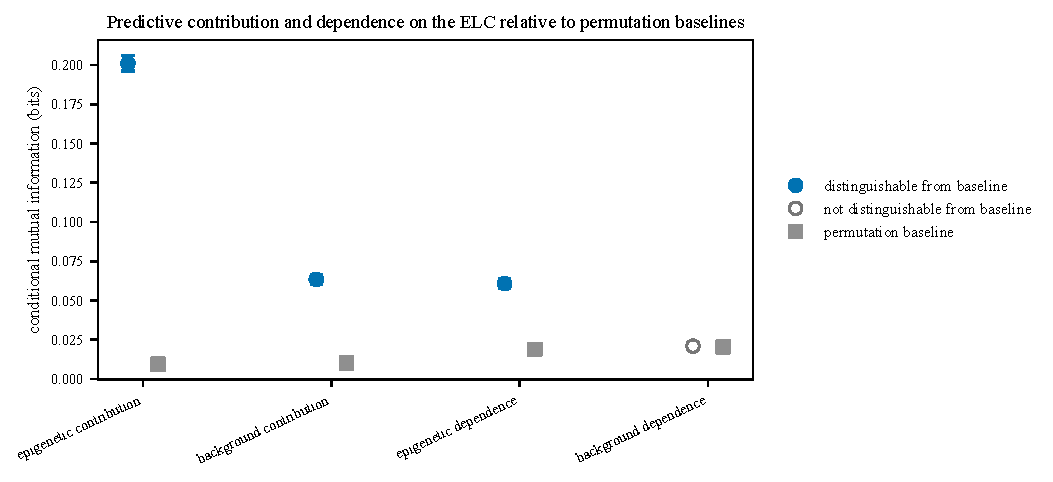
\includegraphics[width=0.86\textwidth]{figure04_predictive_contribution_closure.pdf}
\caption{Predictive contribution and dependence on the ELC. Circles show the estimates with $95\%$ confidence intervals, and squares show the means from $500$ permutations. Filled circles indicate $p\leq0.05$.}
\label{fig:predictive-closure}
\end{figure}

We next evaluated hereditary contributions originating from an additional ELC $d'\neq d$. In the simulation, only the epigenetic level of $d'$ directly influenced the ELC of $d$ through a nonzero $B_{d,d',t_l}^{[l]}$ term. However, because the levels within $d'$ are coupled, other levels of $d'$ may also carry predictive information through their statistical dependence on the epigenetic process. The complete ELC of $d'$ had an estimated transfer entropy of $0.146$ bits, which was $0.0137$ bits ($9.36\%$) above its permutation baseline of $0.133$ bits. The epigenetic level of $d'$ had an estimated transfer entropy of $0.0252$ bits, which was $0.0150$ bits ($59.5\%$) above its permutation baseline of $0.0102$ bits ($p=0.002$ for both; Supplementary Table~S3). We further evaluated the predictive contributions of the individual levels within $d'$ and quantified how this information was distributed across the levels of the next-generation ELC of $d$ (Supplementary Fig.~S4 and Supplementary Table~S4). These findings show that interactions among multiple ELCs can provide hereditary information for the reconstruction of the next-generation ELC, consistent with the expanded account of reproduction \cite{etxeberria2026expanded}.

To evaluate whether the epigenetic factor qualifies as a hereditary unit, we assessed whether it contributed to the reconstruction of a particular phenotypic variant. For this analysis, the epigenetic process provided $0.0212$ bits of predictive information about whether the focal variant $\nu=(1,1)$, corresponding to early maturation with high growth, was reconstructed (Supplementary Table~S5). To establish whether changing the hereditary factor can increase the probability of the variant, we intervened on the epigenetic state and evaluated the resulting changes in the phenotype distribution. The intervention parameters $\theta_{\mathrm{reg}}$ and $\theta_{\mathrm{stress}}$ were each varied over $\{-1.5,-1.0,-0.5,0,0.5,1.0,1.5\}$. These interventions could both increase and decrease the probability of $\nu$. The combination $(\theta_{\mathrm{reg}},\theta_{\mathrm{stress}})=(1.5,-1.5)$ increased $p(\nu)$ by $0.314$, or $31.4$ percentage points, whereas $(-1.5,1.5)$ decreased $p(\nu)$ by $0.328$, or $32.8$ percentage points (Supplementary Fig.~S5 and Supplementary Table~S6). Near $(\theta_{\mathrm{reg}},\theta_{\mathrm{stress}})=(0,0)$, the local gradient was $(0.233,-0.0220)$, indicating that small increases in the regulatory variable and small decreases in the stress-memory variable increased the probability of $\nu$. Fisher information further showed that changes in both epigenetic coordinates altered the probability distribution over the possible phenotypic states, as both diagonal entries of the Fisher information matrix were positive. The epigenetic factor therefore satisfied all three requirements to qualify as a hereditary unit with respect to $\nu$ in $485$ of the $1{,}000$ ELC realizations ($48.5\%$), demonstrating that whether a factor functions as a hereditary unit is context-dependent. 

Our framework also characterized how the epigenetic contribution changed over time within a generation and across successive generations. Within a generation, we evaluated these changes separately at each level of the ELC. The predictive contribution remained distinguishable from the permutation baseline across all five generations evaluated. The estimated information decreased from $0.201$ bits at $\rho=1$ to $0.0251$ bits at $\rho=5$, with $0.192$ bits ($95.3\%$) and $0.0137$ bits ($54.5\%$), respectively, beyond baseline (Figure~\ref{fig:temporal-contribution}; Supplementary Table~S7). Within the next-generation ELC, the contribution was greatest in the developmental GRN and life history levels and smallest in the ecological niche level, and varied across time within those levels (Figure~\ref{fig:temporal-contribution}; Supplementary Table~S8). 

\begin{figure}[H]
\centering

\begin{minipage}{0.72\textwidth}
\centering
\textbf{(a)}\\[0.3em]
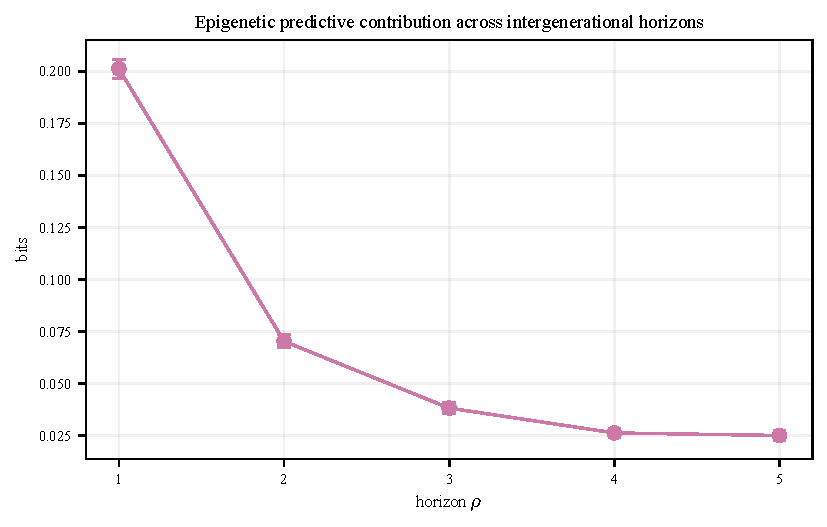
\includegraphics[width=\textwidth]{figure07_intergenerational_stability.pdf}
\end{minipage}

\vspace{0.8em}

\begin{minipage}{0.62\textwidth}
\centering
\textbf{(b)}\\[0.3em]
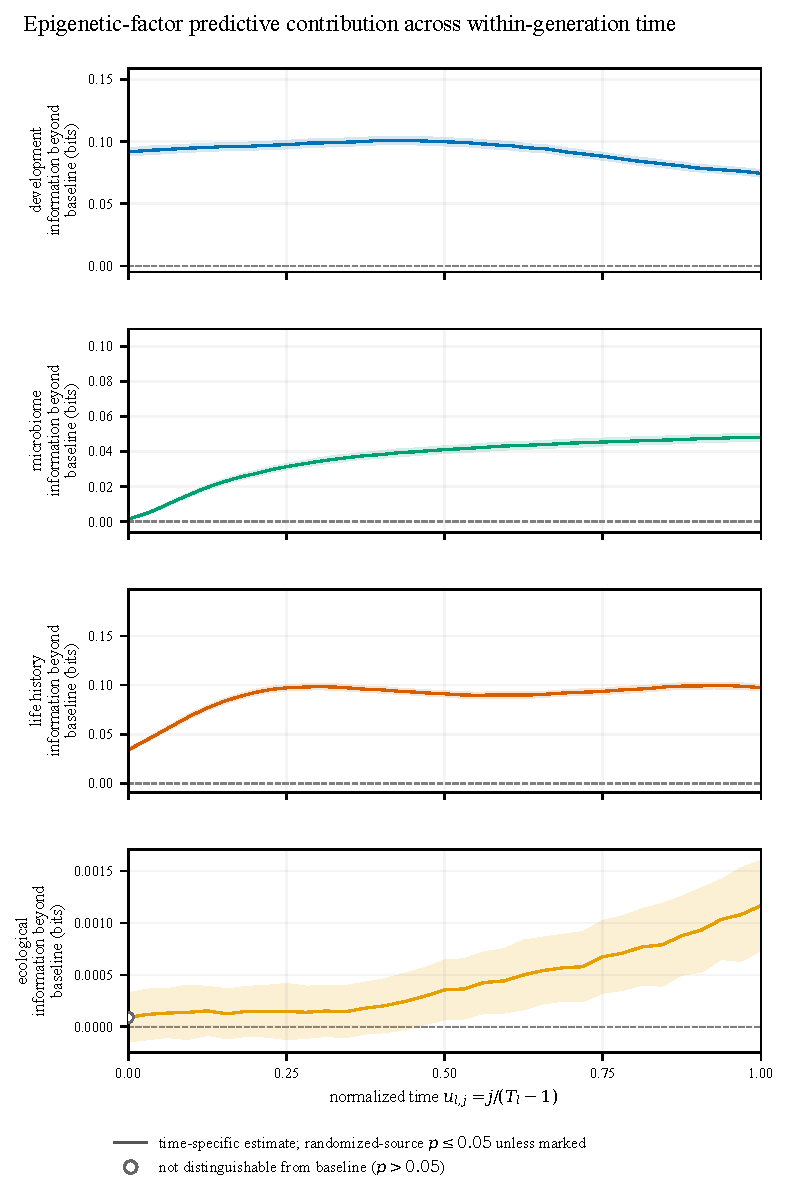
\includegraphics[width=\textwidth]{figure08_level_time_location.pdf}
\end{minipage}

\caption{(a) The epigenetic factor contributes predictive information across five future generations. Points show the estimated information with $95\%$ confidence intervals. (b) The epigenetic factor contributes different amounts of predictive information over normalized time within the next-generation ELC. Lines show information above the permutation baseline, bands show $95\%$ confidence intervals, and open markers indicate $p>0.05$.}
\label{fig:temporal-contribution}
\end{figure}

Finally, we evaluated whether the epigenetic and ecological factors qualified as a complex unit of inheritance. For this analysis, the focal variant was $\nu=(0,0)$, corresponding to non-early maturation and low growth. When considered jointly, the epigenetic and ecological factors contributed $0.284$ bits beyond baseline to the next-generation ELC, and the ELC contributed $0.0867$ bits beyond baseline to their future states ($p=0.002$ for both; Supplementary Table~S12). The factors therefore satisfied Criteria~1-2 in Section~3.2. Partial information decomposition identified $0.0298$ bits of synergistic information, corresponding to $9.79\%$ of the total information in the decomposition (Figure~\ref{fig:complex-unit}a; Supplementary Table~S9). The hereditary factors also provided $0.0274$ bits of predictive information about whether $\nu$ was reconstructed, satisfying Criterion~1 in Section~3.2.1. A phenotype-specific partial information decomposition summed to $0.0270$ bits, of which $0.0110$ bits ($40.8\%$) were available only when both factors were considered jointly (Figure~\ref{fig:complex-unit}b; Supplementary Table~S10). This satisfied the requirement that a complex unit provide synergistic information about the reconstruction of the focal variant. The five intervention parameters corresponded to the regulatory, stress-memory, soil, resource, and microclimate variables. Setting all five parameters to $-0.5$ increased $p(\nu)$ from $0.264$ to $0.590$, an increase of $0.326$, or $32.6$ percentage points (Supplementary Table~S12). Near $\boldsymbol{\theta}=\mathbf{0}$, the local gradient was $(-0.207,0.0168,-0.0265,-0.290,-0.0962)$. Decreasing the regulatory, soil, resource, or microclimate variable, or increasing the stress-memory variable, increased $p(\nu)$. The diagonal entries in the Fisher information matrix were positive for all five intervention parameters, showing that local changes in each parameter altered the phenotype distribution. The epigenetic and ecological factors therefore satisfied Criterion~2 in Section~3.2.1. Their predictive contribution was also distributed across the developmental GRN, microbiome, and life-history levels and varied across time within those levels (Supplementary Fig.~S10 and Supplementary Table~S11). The criteria to qualify as a complex unit of inheritance were met in $455$ of the $1{,}000$ ELC realizations ($45.5\%$).
\begin{figure}[H]
\centering

\begin{minipage}{0.47\textwidth}
\centering
\textbf{(a)}\\[0.3em]
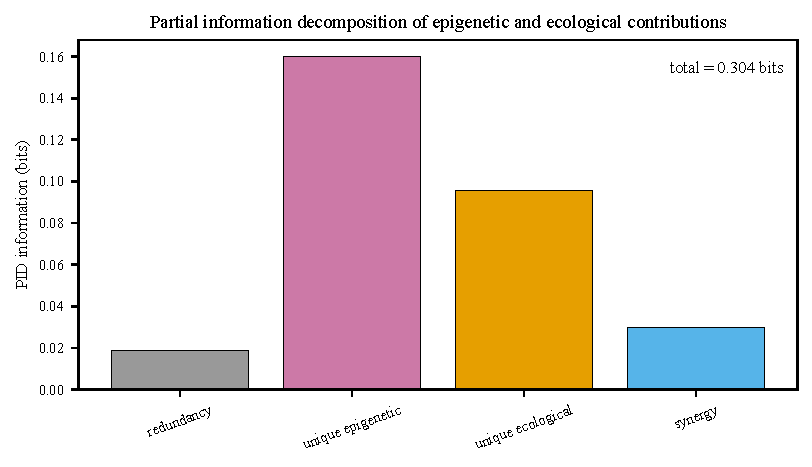
\includegraphics[width=\textwidth]{figure06_epigenetic_ecological_pid.pdf}
\end{minipage}
\hfill
\begin{minipage}{0.47\textwidth}
\centering
\textbf{(b)}\\[0.3em]
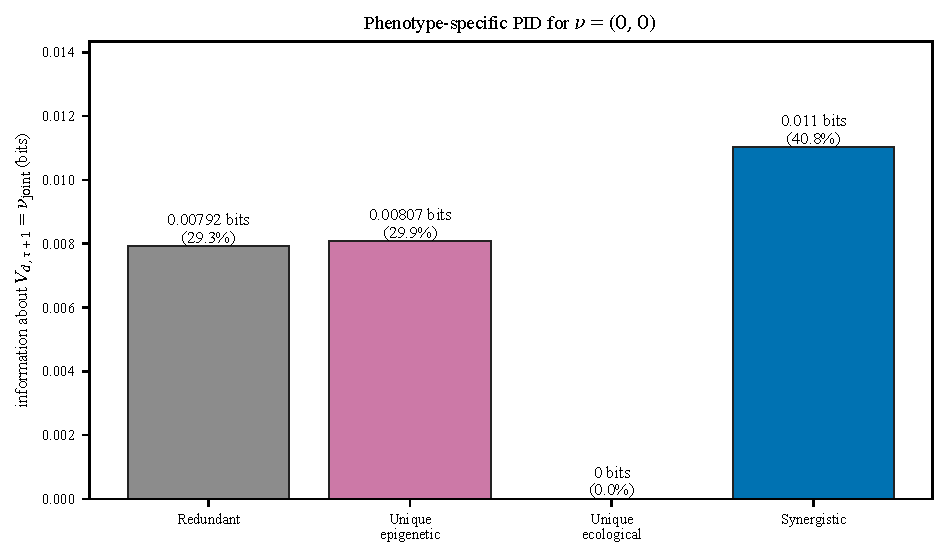
\includegraphics[width=\textwidth]{figure11_joint_variant_00_pid.pdf}
\end{minipage}

\caption{(a) Redundant, unique, and synergistic information contributed by the epigenetic and ecological factors. The four components sum to $0.304$ bits. (b) Redundant, unique, and synergistic information about $\nu=(0,0)$.}
\label{fig:complex-unit}
\end{figure}

\section{Discussion: Implications}
The simulation demonstrates that our information theoretic framework can identify, quantify, and characterize hereditary information as it is generated within and distributed throughout the complex system that is the Extended Life Cycle without privileging particular types of hereditary factors or channels in explanations of the reconstruction of organizational features or specific phenotypic variants. In doing so, our work provides measures for making claims about the parity thesis empirically testable while preserving its central conceptual commitment. Notably, our work presents a departure from non-genetic extensions of the Price equation, which have primarily focused on how genetic and non-genetic inheritance alter the response to selection within populations \cite{day2011unified,helantera2020different}, and from inclusive-heritability and variance-partitioning approaches, which represent genetic and non-genetic inheritance as variance components inferred from resemblance among relatives \cite{danchin2011beyond,thomson2018guide}. By contrast, in directly modeling the multilevel mechanisms constitutive of organismal activities through which hereditary factors are interpreted and made consequential, our framework foregrounds the active role that organisms play in shaping their developmental, reproductive, and evolutionary outcomes through the meaning-making processes by which they exercise their agency. This perspective more directly aligns with the theoretical and explanatory commitments of extended evolutionary theory, and in particular the Extended Evolutionary Synthesis \cite{laland2015extended}, which seeks an organism-centered account of evolution in which organisms are recognized as active causal participants rather than passive objects of evolutionary processes. Several additional philosophical implications emerge as a consequence of our information theoretic framework, which we briefly elaborate below.

\subsection{Linking transmission and organization for organism-centric heredity}
The gene-centric view of heredity posits that the germline is the sole channel through which hereditary information, localized in instructional elements, can be transmitted across generations, while privileging genes as those information-bearing units that are responsible for organismal continuity and parent-offspring resemblances. The success of gene centrism may, in large part, be attributed to the formal operationalizability of the gene concept, around which the mathematical framework of population genetics was built. At the same time, the gene serves as a bridge concept linking heredity, phenotypic variation, and evolutionary change. These conceptual and mathematical contributions, alongside the success of molecular genetics, helped to further establish the legitimacy of the gene and genetics as a formal research program and experimental science. In parallel, with these developments, research from embryology and developmental biology has historically operated under the organicist framework, which emphasizes organization, part-whole relations, and the processual nature of organisms, in part influenced by Whitehead’s process philosophy \cite{whitehead2010process}. Under organicism, one of the primary aims of heredity is to explain the maintenance and reconstruction of biological organization. The information-theoretic approach introduced here unites these perspectives within a formal framework that recognizes the transmission of hereditary resources, enables information to be constructed and emerge during ontogenetic processes, and connects it to the reconstruction of biological organization, subsets and features of which correspond to particular phenotypic variants. This framework is centered on the ELC as a bridge concept connecting development, extended inheritance, reproduction, and population/ecological structures and dynamics that explicitly formulates the organism in terms of its dynamism and multilevel organization—or, as a complex biological system. 

\subsection{Evolution as transformations in complex systems over time}
Notably, the reconstruction of particular phenotypic variants, through which parent-offspring resemblance and thus descent with modification are formalized, consequently yields a notion of evolution as transformations in complex systems over time that can be explicitly connected to fitness consequences, for instance via \cite{lean2014getting}. Although we leave a complete elaboration for future work, our framework enables both the direct modeling of these transformations through dynamic and/or structural changes in the ELC, parameterized by its state-space structure in Equation~\ref{eq:elc-state}. Moreover, we may also account for changes in the possible state-space itself, which we also leave for future elaboration. Such transformations may alter not only the possible states and trajectories of the ELC, but also the natural meaning of hereditary inputs, since the same input may produce a different change in the conditional probability distribution over possible next-generation ELC states as the organization of the ELC changes. 

\subsection{The \textit{umwelt} and organismal agency}
Lastly, the ELC can be viewed as providing a mathematical basis for formalizing an organism’s \textit{umwelt}, which is understood as its historically contingent, relationally constituted, and meaningful world shaped by its perceptual capacities, organization, and activities, and is continuously updated as a space of possibilities for experience and action \cite{uexkull2010foray,wolfe2026organisms, sharov2026semiotic, svorcova2026evolution}. This interpretation places our information-theoretic description of extended heredity at the intersection of physical dynamics and biological meaning, where our state-space formalization describes the coupled processes through which the ELC changes over time, while the information-theoretic framework identifies which differences become consequential within the ELC’s evolving space of possibilities. Meaning arises from the roles these variations play within the organized and ongoing activities of the organism. Organismal agency can therefore be understood as the organism’s capacity to act within and modify this space of possibilities, thereby continually reshaping the relations through which its \textit{umwelt} is constituted. Our work therefore aligns with recent initiatives aimed at further developing formal methodologies to study biosemiotic processes across different systems \cite{maekivi2026methodological, vega2024cell, cerrone2021zoosemiotic}.

\section{Conclusion}
In this work, we developed an information-theoretic framework for identifying, quantifying, and characterizing hereditary information within the Extended Life Cycle. Our framework provides criteria for distinguishing hereditary factors from life-enabling background conditions. It also provides measures for identifying hereditary units associated with the reconstruction of particular phenotypic variants and for quantifying the magnitude and intergenerational stability of their contributions. Finally, our framework characterizes how hereditary information is distributed throughout the ELC and provides a means of characterizing the informational contributions of complex units of inheritance through synergistic information. In doing so, the framework brings transmission- and organization-centered approaches to heredity into a common formal structure while maintaining the ELC as an operationalizable bridge concept connecting reproduction, development, extended inheritance, evolutionary change. 

Several directions for future work follow from the present framework. First, empirical applications are needed to evaluate  inheritance processes across different biological systems, levels of organization, and inheritance channels. Such applications will require methods for estimating the latent states and trajectories of the ELC from noisy and partially observed measurements. Second, as the complex system that is the ELC undergoes evolutionary transformations, such transformations not only alter the future states and trajectories of the ELC, but they alter the state-space of possibilities itself. Although this presents a challenge from a modeling standpoint, there are possible avenues that merit further exploration. For instance, open-universe probabilistic modeling permits uncertainty in which and how many entities of pre-specified types exist, thereby allowing the dimensionality of the latent state representation to vary across possible worlds \cite{milch2005blog}. By assigning probabilities to worlds containing different sets and numbers of entities, these models support posterior inference over alternative compositions of a system. Bayesian non-parametric methods can complement open-universe modeling by allowing the number of latent states used to represent the system's dynamics to be inferred from data and need not be specified a priori \cite{tonekaboni2025hdpflow}. 

\begin{thebibliography}{99}

\bibitem{schrodinger2012life}
Erwin Schr\"odinger.
\textit{What Is Life? With Mind and Matter and Autobiographical Sketches}.
Cambridge University Press, 2012.

\bibitem{griffiths2017genetic}
Paul E. Griffiths.
"Genetic, Epigenetic and Exogenetic Information in Development and Evolution."
\textit{Interface Focus}, 7(5):20160152, 2017.


\bibitem{milch2005blog}
Milch, B., Marthi, B., Russell, S., Sontag, D., Ong, D. L., and Kolobov, A. (2005).
BLOG: Probabilistic models with unknown objects.
In \textit{Proceedings of the Nineteenth International Joint Conference on Artificial Intelligence}, 1352--1359.


\bibitem{wolfe2026organisms}
Wolfe, C. (2026).
Organisms as meaning-makers.
In K. Kull and D. Favareau (Eds.),
\textit{Towards a Biosemiotic Theoretical Biology: Sign Processes and Meaning-Making in Living Systems}
(pp. 45--62).
The MIT Press.
\url{https://doi.org/10.7551/mitpress/16007.003.0007}

\bibitem{mediano2022greater}
Mediano, P. A. M., Rosas, F. E., Luppi, A. I., Jensen, H. J., Seth, A. K., Barrett, A. B., Carhart-Harris, R., \& Bor, D. (2022).
Greater than the parts: A review of the information decomposition approach to causal emergence.
\textit{Philosophical Transactions of the Royal Society A: Mathematical, Physical and Engineering Sciences}, \textit{380}(2227), 20210246.

\bibitem{sharov2026semiotic}
Sharov, A. A. (2026).
Semiotic agency: Life is meaning-making.
In K. Kull and D. Favareau (Eds.),
\textit{Towards a Biosemiotic Theoretical Biology: Sign Processes and Meaning-Making in Living Systems}
(pp. 95--112).
The MIT Press.
\url{https://doi.org/10.7551/mitpress/16007.003.0011}

\bibitem{graveley2011developmental}
Graveley, B. R., Brooks, A. N., Carlson, J. W., Duff, M. O., Landolin, J. M.,
Yang, L., Artieri, C. G., Van Baren, M. J., Boley, N., Booth, B. W.,
Brown, J. B., Cherbas, L., Davis, C. A., Dobin, A., Li, R., Lin, W.,
Malone, J. H., Mattiuzzo, N. R., Miller, D., et al. (2011).
The developmental transcriptome of \textit{Drosophila melanogaster}.
\textit{Nature}, \textit{471}, 473--479.
https://doi.org/10.1038/nature09715.

\bibitem{stolc2004gene}
Stolc, V., Gauhar, Z., Mason, C., Halasz, G., van Batenburg, M. F., Rifkin, S. A., Hua, S., Herreman, T., Tongprasit, W., Barbano, P. E., Bussemaker, H. J., \& White, K. P. (2004).
A gene expression map for the euchromatic genome of \textit{Drosophila melanogaster}.
\textit{Science}, \textit{306}(5696), 655--660.
https://doi.org/10.1126/science.1101312.

\bibitem{todorov2024stage}
Todorov, H., Wei{\ss}bach, S., Schlichtholz, L., Mueller, H., Hartwich, D., Gerber, S., \& Winter, J. (2024).
Stage-specific expression patterns and co-targeting relationships among miRNAs in the developing mouse cerebral cortex.
\textit{Communications Biology}, \textit{7}, 1366.
https://doi.org/10.1038/s42003-024-07092-7.

\bibitem{tonekaboni2025hdpflow}
Tonekaboni, S., Behrouzi, T., Weatherhead, A., Fox, E., Blei, D., and Goldenberg, A. (2025).
HDP-Flow: Generalizable Bayesian nonparametric model for time series state discovery.
In \textit{Proceedings of the Forty-First Conference on Uncertainty in Artificial Intelligence},
\textit{Proceedings of Machine Learning Research}, 286, 4227--4250.

\bibitem{svorcova2026evolution}
\v{S}vorcov\'a, J., and Kleisner, K. (2026).
Evolution by habits: Organismal organization beyond natural selection.
In K. Kull and D. Favareau (Eds.),
\textit{Towards a Biosemiotic Theoretical Biology: Sign Processes and Meaning-Making in Living Systems}
(pp. 141--158).
The MIT Press.
\url{https://doi.org/10.7551/mitpress/16007.003.0015}

\bibitem{jablonka2019systemic}
Jablonka, E., \& Noble, D. (2019).
Systemic integration of different inheritance systems.
\textit{Current Opinion in Systems Biology}, \textit{13}, 52--58.
https://doi.org/10.1016/j.coisb.2018.10.002.

\bibitem{martinez2018multimodal}
Martinez, A. J., Doremus, M. R., Kraft, L. J., Kim, K. L., \& Oliver, K. M. (2018).
Multi-modal defences in aphids offer redundant protection and increased costs likely impeding a protective mutualism.
\textit{Journal of Animal Ecology}, \textit{87}(2), 464--477.
https://doi.org/10.1111/1365-2656.12675.

\bibitem{crick1958protein}
Francis H. C. Crick.
"On Protein Synthesis."
In \textit{The Biological Replication of Macromolecules},
\textit{Symposia of the Society for Experimental Biology},
vol.~12, pp.~138--163.
Cambridge University Press, 1958.

\bibitem{keller2009rethinking}
Evelyn Fox Keller.
"Rethinking the Meaning of Biological Information."
\textit{Biological Theory}, 4(2):159--166, 2009.

\bibitem{rama2026probabilistic}
Tiago Rama.
"Probabilistic Epigenetics: An Informational Approach."
\textit{Synthese}, 207(3):130, 2026.

\bibitem{gutzwiller2015dynamics}
Gutzwiller, F., Carmo, C. R., Miller, D. E., Rice, D. W., Newton, I. L. G.,
Hawley, R. S., Teixeira, L., \& Bergman, C. M. (2015).
Dynamics of \textit{Wolbachia pipientis} gene expression across the
\textit{Drosophila melanogaster} life cycle.
\textit{G3: Genes|Genomes|Genetics}, \textit{5}(12), 2843--2856.
https://doi.org/10.1534/g3.115.021931.

\bibitem{isaac2019semantics}
Alistair M. C. Isaac.
"The Semantics Latent in Shannon Information."
\textit{The British Journal for the Philosophy of Science},
70(1):103--125, 2019.


\bibitem{williams2010nonnegative}
Paul L. Williams and Randall D. Beer.
"Nonnegative Decomposition of Multivariate Information."
\textit{arXiv preprint arXiv:1004.2515}, 2010.

\bibitem{whitehead2010process}
Alfred North Whitehead.
\textit{Process and Reality}.
Simon and Schuster, 2010.

\bibitem{rama2026developmental}
Tiago Rama.
"Developmental Synergistic Information."
\textit{Theory in Biosciences}, 145(3):23, 2026.

\bibitem{scarantino2015information}
Andrea Scarantino.
"Information as a Probabilistic Difference Maker."
\textit{Australasian Journal of Philosophy},
93(3):419--443, 2015.

\bibitem{jablonka2002information}
Eva Jablonka.
"Information: Its Interpretation, Its Inheritance, and Its Sharing."
\textit{Philosophy of Science}, 69(4):578--605, 2002.

\bibitem{pontarotti2015extended}
Ga\"{e}lle Pontarotti.
"Extended Inheritance from an Organizational Point of View."
\textit{History and Philosophy of the Life Sciences},
37(4):430--448, 2015.

\bibitem{day2011unified}
Day, T. \& Bonduriansky, R. A unified approach to the evolutionary consequences of genetic and nongenetic inheritance. \textit{The American Naturalist} \textbf{178}, E18--E36 (2011).

\bibitem{helantera2020different}
Helanter\"{a}, H. \& Uller, T. Different perspectives on non-genetic inheritance illustrate the versatile utility of the Price equation in evolutionary biology. \textit{Philosophical Transactions of the Royal Society B: Biological Sciences} \textbf{375}, 20190366 (2020).

\bibitem{danchin2011beyond}
Danchin, E., Charmantier, A., Champagne, F. A., Mesoudi, A., Pujol, B. \& Blanchet, S. Beyond DNA: integrating inclusive inheritance into an extended theory of evolution. \textit{Nature Reviews Genetics} \textbf{12}, 475--486 (2011).

\bibitem{thomson2018guide}
Thomson, C. E., Winney, I. S., Salles, O. C. \& Pujol, B. A guide to using a multiple-matrix animal model to disentangle genetic and nongenetic causes of phenotypic variance. \textit{PLoS ONE} \textbf{13}, e0197720 (2018).

\bibitem{mossio2022conserving}
Matteo Mossio and Ga\"{e}lle Pontarotti.
"Conserving Functions across Generations: Heredity in Light of Biological Organization."
\textit{The British Journal for the Philosophy of Science},
73(1):249--278, 2022.

\bibitem{kolchinsky2022novel}
Kolchinsky, A.
A novel approach to the partial information decomposition.
\textit{Entropy} \textbf{24}, 403 (2022).

\bibitem{moore2019mothers}
Moore, M. P., Whiteman, H. H., \& Martin, R. A. (2019).
A mother's legacy: the strength of maternal effects in animal populations.
\textit{Ecology Letters}, \textit{22}(10), 1620--1628.
https://doi.org/10.1111/ele.13351.

\bibitem{yang2020msh1}
Yang, X., Sanchez, R., Kundariya, H., Maher, T., Dopp, I., Schwegel, R., Virdi, K., Axtell, M. J., \& Mackenzie, S. A. (2020).
Segregation of an MSH1 RNAi transgene produces heritable non-genetic memory in association with methylome reprogramming.
\textit{Nature Communications}, \textit{11}, 2214.
https://doi.org/10.1038/s41467-020-16036-8.

\bibitem{shahmohamadloo2025transgenerational}
Shahmohamadloo, R. S., Fryxell, J. M., \& Rudman, S. M. (2025).
Transgenerational epigenetic inheritance increases trait variation but is not adaptive.
\textit{Evolution}, \textit{79}(6), 1033--1043.
https://doi.org/10.1093/evolut/qpaf050.

\bibitem{lyu2026multivariate}
Lyu, A., Clark, A. \& Raviv, N.
Multivariate partial information decomposition: Constructions, inconsistencies, and alternative measures.
\textit{Physical Review E} \textbf{113}, 034102 (2026).

\bibitem{veigl2022rethinking}
Sophie J. Veigl, Javier Su\'arez, and Adrian Stencel.
"Rethinking Hereditary Relations: The Reconstitutor as the Evolutionary Unit of Heredity."
\textit{Synthese}, 200(5):367, 2022.

\bibitem{bruno2026stochastic}
Simone Bruno and Domitilla Del Vecchio.
"Stochastic Modeling of Epigenetic Memory."
\textit{npj Systems Biology and Applications}, 12(1):58, 2026.

\bibitem{prigent2026ecological}
Iris Prigent and Charles Mullon.
"Ecological Inheritance Facilitates the Coexistence of Environmental Helpers and Free Riders."
\textit{Proceedings of the National Academy of Sciences},
123(9):e2527016123, 2026.

\bibitem{lean2014getting}
Lean, O. M. (2014).
"Getting the most out of Shannon information."
\textit{Biology \& Philosophy}, 29(3), 395--413.

\bibitem{montevil2015biological}
Mont{\'e}vil, M. and Mossio, M. (2015).
Biological organisation as closure of constraints.
\textit{Journal of Theoretical Biology}, 372, 179--191.

\bibitem{pocheville2017crick}
Arnaud Pocheville, Ma\"el Mont\'evil, Karola Stotz, and Paul E. Griffiths.
"Crick Information: Giving Substance to Biological Information."
Unpublished manuscript, March 12, 2017.

\bibitem{calcott2014creation}
Brett Calcott.
"The Creation and Reuse of Information in Gene Regulatory Networks."
\textit{Philosophy of Science}, 81(5):879--890, 2014.

\bibitem{maynardsmith2000information}
John Maynard Smith.
"The Concept of Information in Biology."
\textit{Philosophy of Science}, 67(2):177--194, 2000.

\bibitem{bonduriansky2020extended}
Russell Bonduriansky and Troy Day.
\textit{Extended Heredity: A New Understanding of Inheritance and Evolution}.
Princeton University Press, 2020.

\bibitem{laland2015extended}
Laland, K. N., Uller, T., Feldman, M. W., Sterelny, K., M{\"u}ller, G. B., Moczek, A., Jablonka, E. \& Odling-Smee, J. The extended evolutionary synthesis: its structure, assumptions and predictions. \textit{Proceedings of the Royal Society B: Biological Sciences} \textbf{282}, 20151019 (2015).

\bibitem{bober1991muscle}
Eva Bober, G. E. Lyons, Thomas Braun, Giulio Cossu, Margaret Buckingham,
and Hans-Henning Arnold.
"The Muscle Regulatory Gene, Myf-6, Has a Biphasic Pattern of Expression during Early Mouse Development."
\textit{The Journal of Cell Biology}, 113(6):1255--1265, 1991.

\bibitem{velez2026extended}
Nayely V\'elez-Cruz and Manfred D. Laubichler.
"The Extended Life Cycle: A Multilevel--Multiscale Modelling Framework for Extended Evolutionary Dynamics."
\textit{Royal Society Open Science}, 13(1), 2026.


\bibitem{griffiths2015measuring}
Paul E. Griffiths, Arnaud Pocheville, Brett Calcott, Karola Stotz,
Hyunju Kim, and Rob Knight.
"Measuring Causal Specificity."
\textit{Philosophy of Science}, 82(4):529--555, 2015.

\bibitem{maekivi2026methodological}
Nelly M{\"a}ekivi and Jana {\v{S}}vorcov{\'a}.
"On the Methodological Foundations of Biosemiotics."
\textit{Biosemiotics}, 2026:1--26, 2026.

\bibitem{vega2024cell}
Federico Vega.
"The cell as a semiotic system that realizes closure to efficient causation:
The semiotic (M, R) system."
\textit{BioSystems}, 240:105226, 2024.

\bibitem{etxeberria2026expanded}
Arantza Etxeberria and David Cort\'es-Garc\'ia.
"Toward Expanded Reproduction: An Intraorganismal and Interorganismal Relational Account."
In Kalevi Kull and Donald Favareau, editors,
\textit{Towards a Biosemiotic Theoretical Biology: Sign Processes and Meaning-Making in Living Systems},
pp.~175--190.
MIT Press, Cambridge, MA, 2026.

\bibitem{saavedra2013chronic}
Lorena Saavedra-Rodr\'{\i}guez and Larry A. Feig.
"Chronic Social Instability Induces Anxiety and Defective Social Interactions across Generations."
\textit{Biological Psychiatry}, 73(1):44--53, 2013.

\bibitem{lizier2014jidt}
Joseph T. Lizier.
"JIDT: An Information-Theoretic Toolkit for Studying the Dynamics of Complex Systems."
\textit{Frontiers in Robotics and AI}, 1:11, 2014.

\bibitem{barad2007meeting}
Karen Barad.
\textit{Meeting the Universe Halfway: Quantum Physics and the Entanglement of Matter and Meaning}.
Duke University Press, 2007.

\bibitem{paaby2014cryptic}
Annalise B. Paaby and Matthew V. Rockman.
"Cryptic Genetic Variation: Evolution's Hidden Substrate."
\textit{Nature Reviews Genetics}, 15(4):247--258, 2014.

\bibitem{levy2011information}
Arnon Levy.
"Information in Biology: A Fictionalist Account."
\textit{No\^{u}s}, 45(4):640--657, 2011.

\bibitem{shea2007representation}
Nicholas Shea.
"Representation in the Genome and in Other Inheritance Systems."
\textit{Biology \& Philosophy}, 22(3):313--331, 2007.

\bibitem{bergstrom2011transmission}
Carl T. Bergstrom and Martin Rosvall.
"The Transmission Sense of Information."
\textit{Biology \& Philosophy}, 26(2):159--176, 2011.

\bibitem{heard2014transgenerational}
Edith Heard and Robert A. Martienssen.
"Transgenerational Epigenetic Inheritance: Myths and Mechanisms."
\textit{Cell}, 157(1):95--109, 2014.
doi:10.1016/j.cell.2014.02.045.


\bibitem{dejong2002modeling}
de Jong, H.
Modeling and simulation of genetic regulatory systems: a literature review.
\textit{Journal of Computational Biology} \textbf{9}, 67--103 (2002).
doi:10.1089/10665270252833208.

\bibitem{stein2013ecological}
Stein, R. R. et al.
Ecological modeling from time-series inference: insight into dynamics and stability of intestinal microbiota.
\textit{PLoS Computational Biology} \textbf{9}, e1003388 (2013).
doi:10.1371/journal.pcbi.1003388.

\bibitem{bucci2016mdsine}
Bucci, V. et al.
MDSINE: Microbial dynamical systems inference engine for microbiome time-series analyses.
\textit{Genome Biology} \textbf{17}, 121 (2016).
doi:10.1186/s13059-016-0980-6.

\bibitem{uexkull2010foray}
Jakob von Uexk{\"u}ll.
\textit{A Foray into the Worlds of Animals and Humans: With A Theory of Meaning}.
Translated by Joseph D. O'Neil.
University of Minnesota Press, Minneapolis, 2010.

\bibitem{velezcruz2026elc}
Nayely Vélez-Cruz and Manfred D. Laubichler.
"The Extended Life Cycle as a Bridge Concept for Contemporary Evolutionary Theory."
Manuscript submitted for publication, 2026.

\bibitem{quadrana2016plant}
Leandro Quadrana and Vincent Colot.
"Plant Transgenerational Epigenetics."
\textit{Annual Review of Genetics}, 50:467--491, 2016.
doi:10.1146/annurev-genet-120215-035254.

\bibitem{cerrone2021zoosemiotic}
Mirko Cerrone and Nelly M{\"a}ekivi.
"A zoosemiotic approach to the transactional model of communication."
\textit{Semiotica}, 2021(242):39--62, 2021.
\end{thebibliography}

\end{document}
